\documentclass[a4paper,12pt,leqno]{report}
\title{Torpedo ROV Report}
\usepackage[options]{xcolor}
\usepackage[margin=1in]{geometry}
\usepackage[backgroundcolor=yellow!40,outlinewidth = 3cm]{mdframed}
\usepackage[T1]{fontenc}
\usepackage{tgbonum}
\usepackage{float}
\usepackage{wrapfig}
\usepackage[options]{graphicx}
%\usepackage[backgroundcolor = yellow!30,outlinewidth = 3cm]{mdframed}
\usepackage[options]{pdfpages}
\usepackage{fancyhdr}
\pagestyle{fancy}
\begin{document}
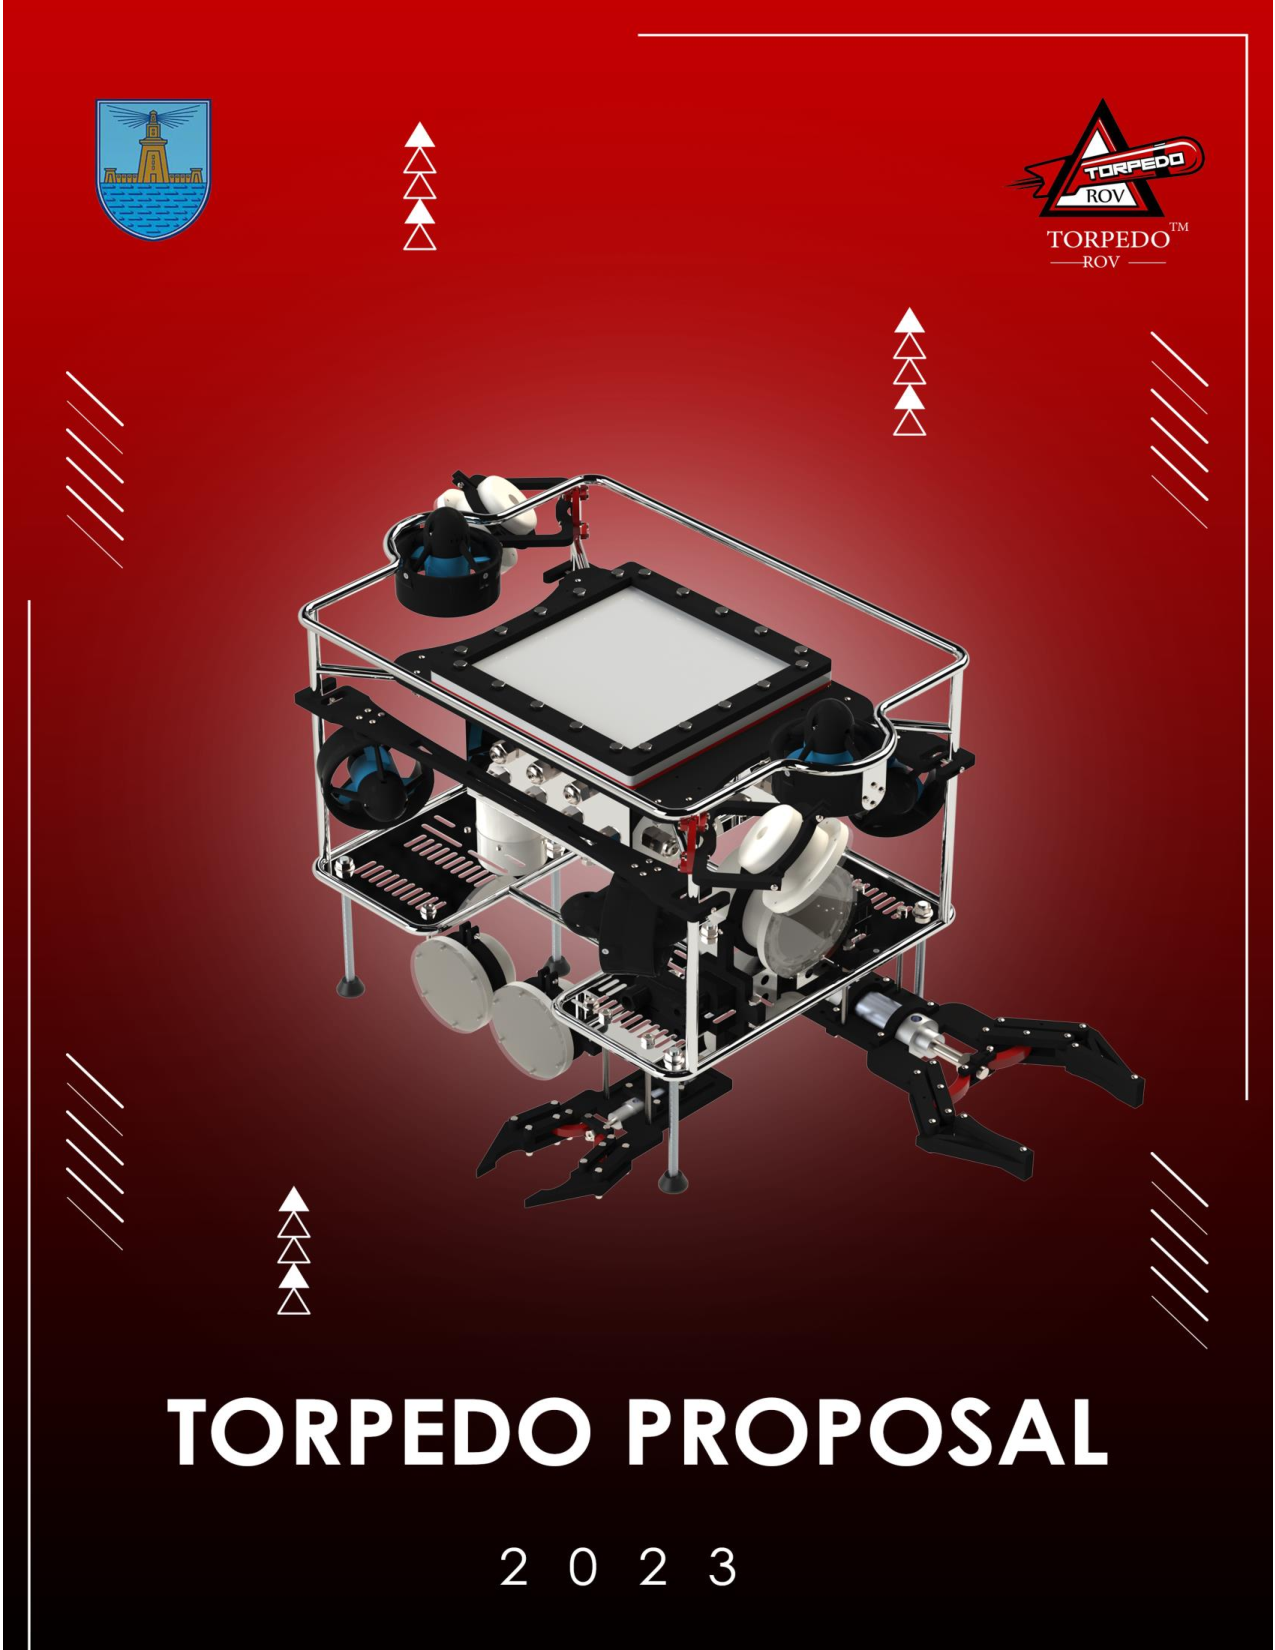
\includepdf[page=1,fitpaper]{Cover_Page}
\tableofcontents
\fancyhf{}
\renewcommand{\headrulewidth}{0pt}
\setlength{\headsep}{1.5cm}
\fancyhead[L]{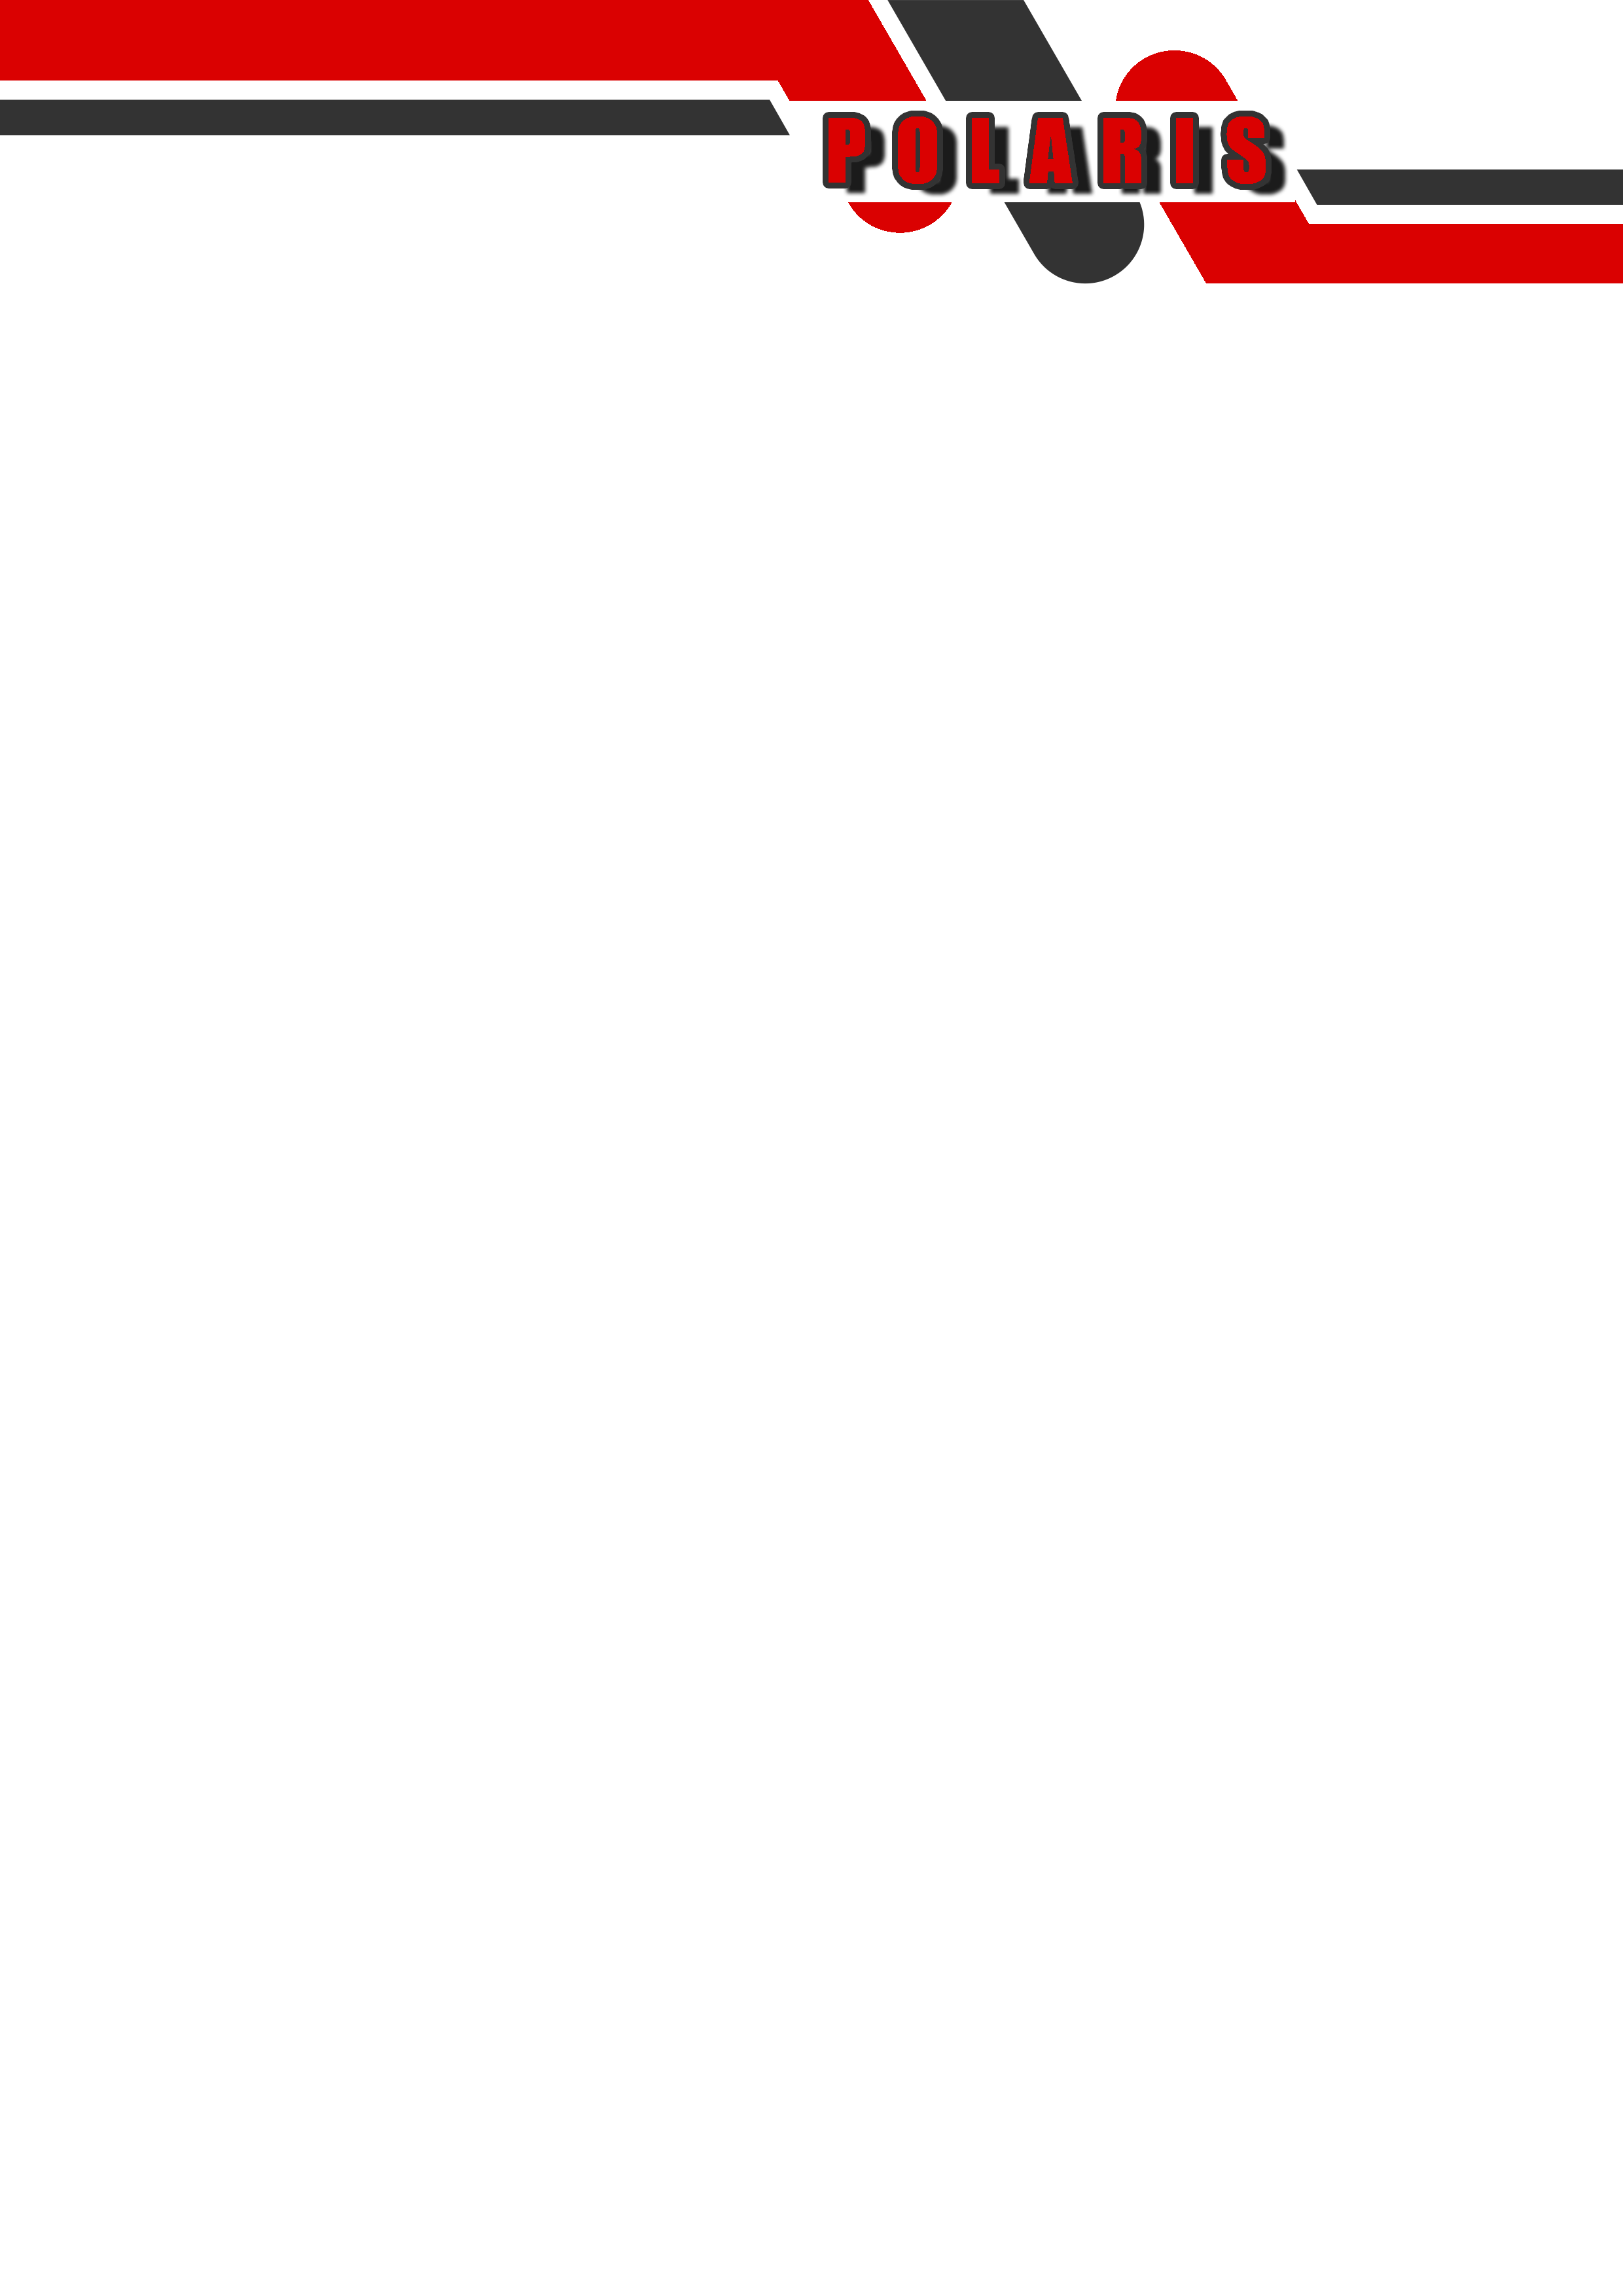
\includegraphics[width=\textwidth, height = .45\textheight]{header}}
\fancyfoot{} 
\fancyfoot[C]{\thepage}

\newpage
\textcolor{red!60}{
\section{Abstract}}
We are tied to the ocean. And when we go back to the sea, whether it is to sail or to watch, we  are going back from whence we came.” — John F. Kennedy For 9 years, Torpedo has aimed to provide individuals with the right ambition, passion,  innovation, and skills to explore our homeland Egypt which overlooks two wonderful seas: the red sea and the Mediterranean. 
And so, after rough days and long nights of brainstorming,  
designing, prototyping, and fabrication, we are proud to reveal our  
newest product, Polaris. 
Our ROV is named after the north pole star, and as sailors used it  
to illuminate their darkness, Polaris is going to be the centerpiece of our set of ROV’s, proving our dedication to the field. 
We started designing Polaris with the help of CAD software   
(Solid Works), equipping it with 2 manipulators to achieve high  functionality, and six Blue Robotics T-200 thrusters which give high  efficiency at low cost. 
When delivering Polaris, we made sure it met all safety standards and the required specifications, making it ready for field work. This document illustrates the technical abilities of our final system, and decisions made throughout the development process. It also shows how  our project management methodology has helped us achieve our goal in the most effective wiz possible. \\
\textcolor{red!60}{
\section{Design Rational}}
\textcolor{blue!90}{
\subsection{Mechanical System}}
\textcolor{blue!40}{
\subsubsection{A- Design Evaluation}}
\begin{figure}[H]
	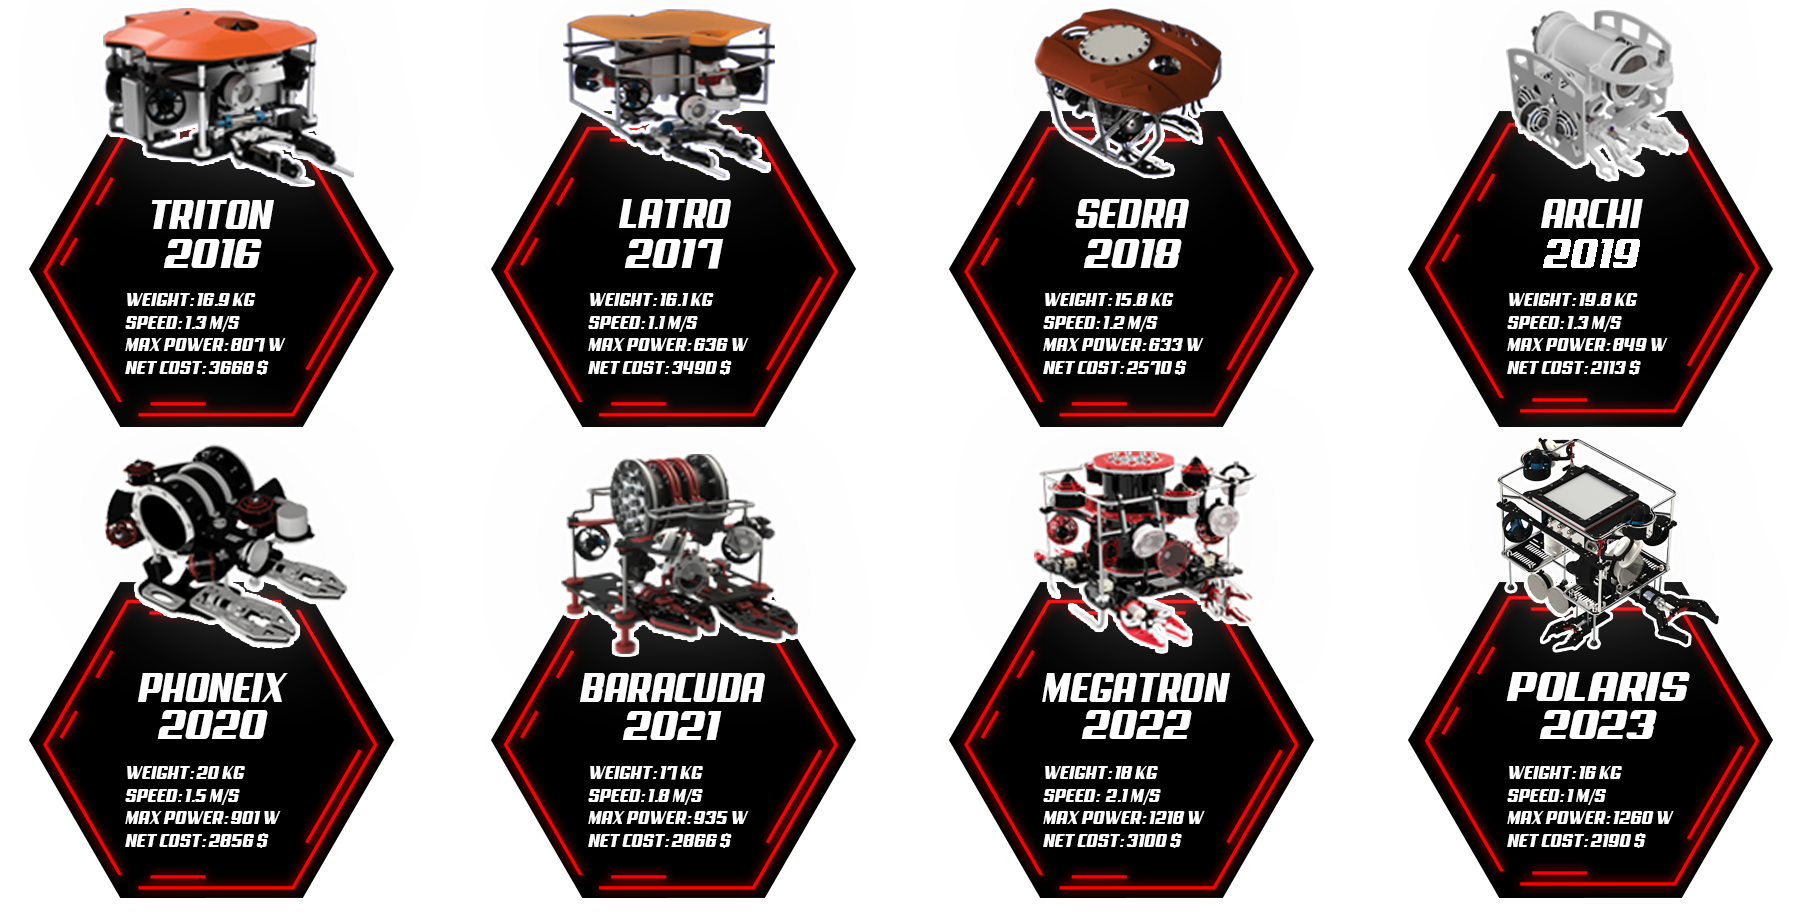
\includegraphics[width=\textwidth]{Design_Evaluation}
\end{figure}

Before starting the process, we wanted to make sure the team had the adequate knowledge to embark on this adventure, and so a training phase was allocated, where the old members  passed on all their knowledge and experience to the new members. 
After the training phase, we begun the brainstorming phase, where we held several meetings,  attended by both the old and new members. We started thinking of solutions to problems we faced before, improvements we can add to our system, and a way to integrate these ideas  together. We decided to reuse previous designs due to their proven performance, in addition to  avoiding the problems we had faced before and adding new features we had thought of before,At the end, we came out with Polaris,\linebreak  an ROV which topped all our previous products, passed  all safety and quality standards, and satisfied industrial requirements.
\\
\textcolor{blue!40}{
\subsubsection{B- Innovation System }}
\begin{table}[H]
	\centering
\caption{Innovation System }
\begin{tabular}{|p{7cm}|p{7cm}|}
	\hline
\textcolor{red!80}{Mechanical}&\textcolor{red!80}{Electrical}\\ \hline
	Compact and light frame & Inserting leakage sensors in our box \\ \hline
	Flexible camera fixations with multiple view.&bullet connectors to connect the ESC’s to thrusters. \\ \hline 
	Pneumatic levels of gripper. & Using an ESP32 as our main controller.\\ \hline
	Manually rotating gripper. &\\ \hline
	Assembled electronics house structure  for easy maintenance.& \\ \hline
\end{tabular}
\end{table}
\textcolor{blue!40}{
\subsubsection{C- Mechanical Structure}}
This year, the design focused on three main goals: improving stability,  making better use of spaces, and molecularity, all while taking in the manufacturing process in mind.\\
	\begin{wrapfigure}{r}{.4\textwidth}
		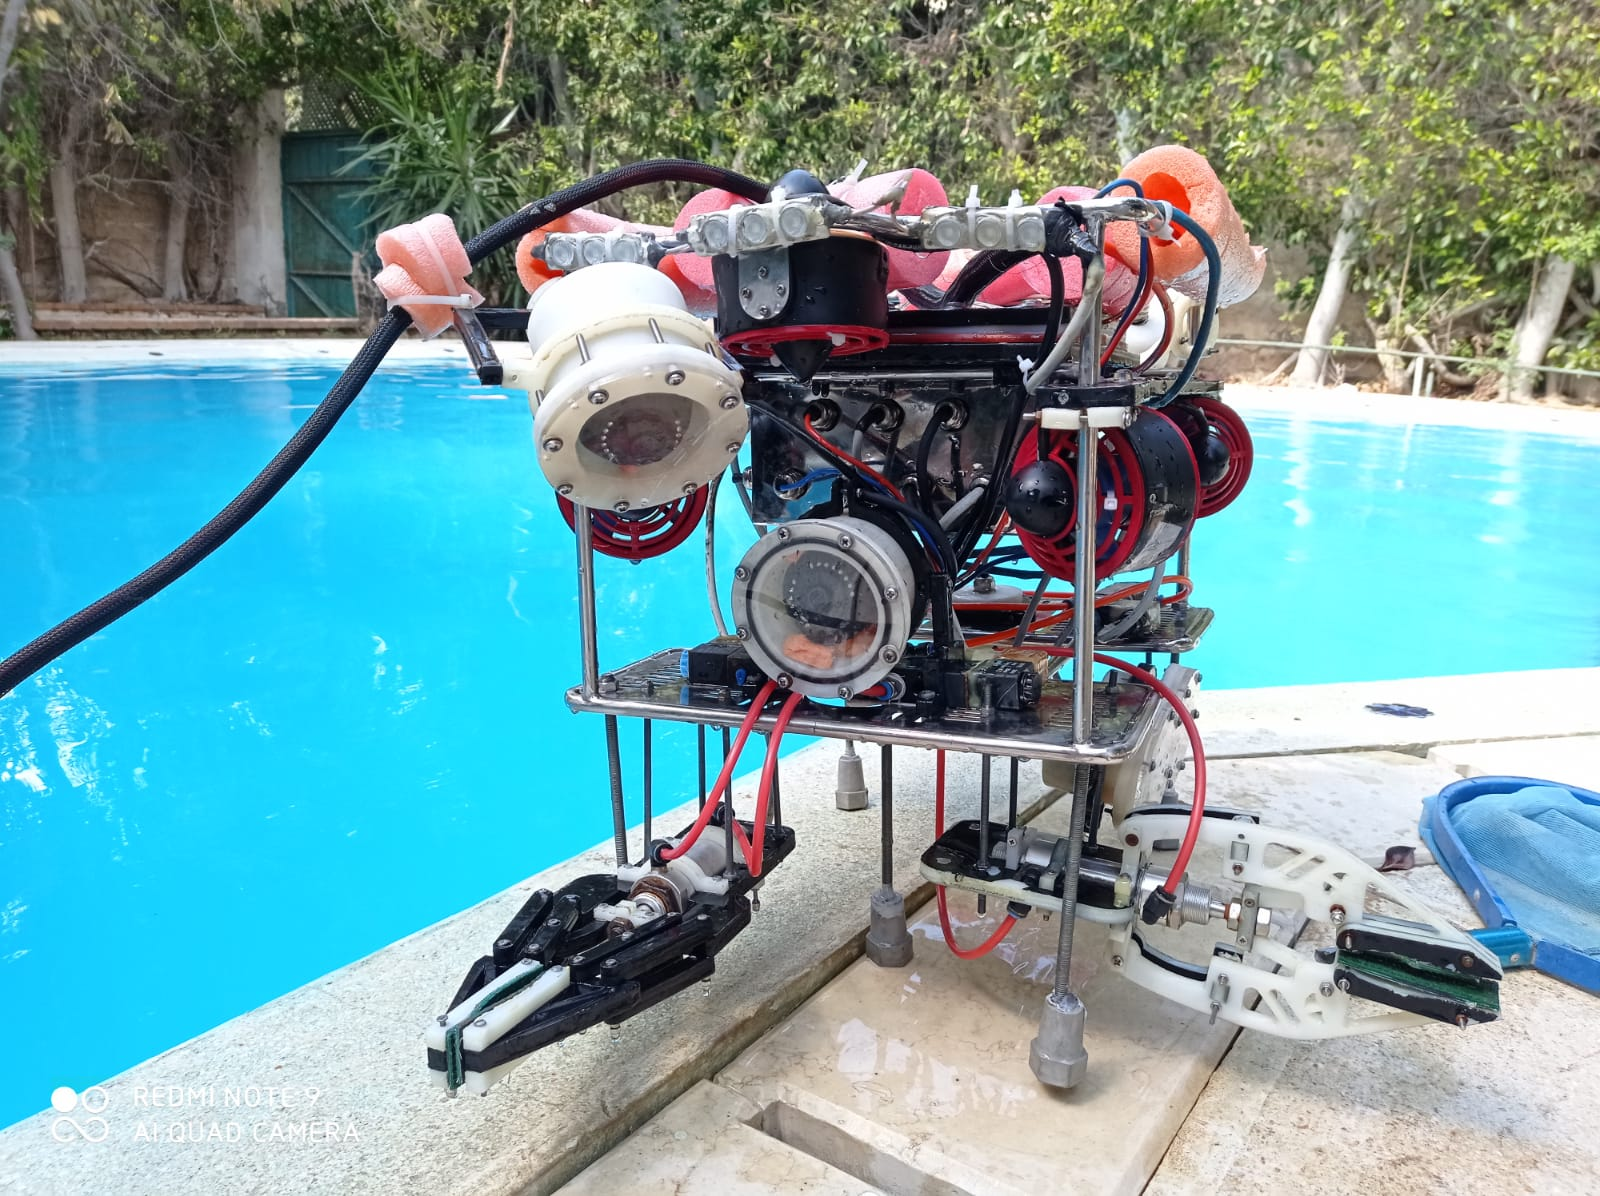
\includegraphics[width= .4\textwidth,height= .16\textheight]{Isometric view-1}
		\caption{Polaris.}
	\end{wrapfigure} 
\textcolor{orange!60}{
\subsubsection{1- Frame}}
The frame consists of a structure made of stainless-steel tubes and  four plates, two of which are of HDPE material, which are fixed to  the sides and are responsible for fixing the thrusters. This design  allows us to change the level of  thrusters to make the center of  thrust at the same level as the center of drag, which ensures the  horizontal stability of the vehicle. The other two are responsible for  installing the rest of the tools, and are also made of stainless steel,  which is resistant to rust, to provide high durability and reduced weight. This design allows us to control the position of  tools in  two different directions and gives us the ability to lower the center  of gravity of the vehicle (which improves balance), ensures the  stability of  tools during operation, and eases dismantlement,which in turn simplifies the maintenance process. To keep these tools at a high level, we  used the help of topology science this year to make the design cost-effective. Moreover, stress analysis was made to ensure frame strength.\\
\begin{wrapfigure}{r}{.4\textwidth}
	\centering
	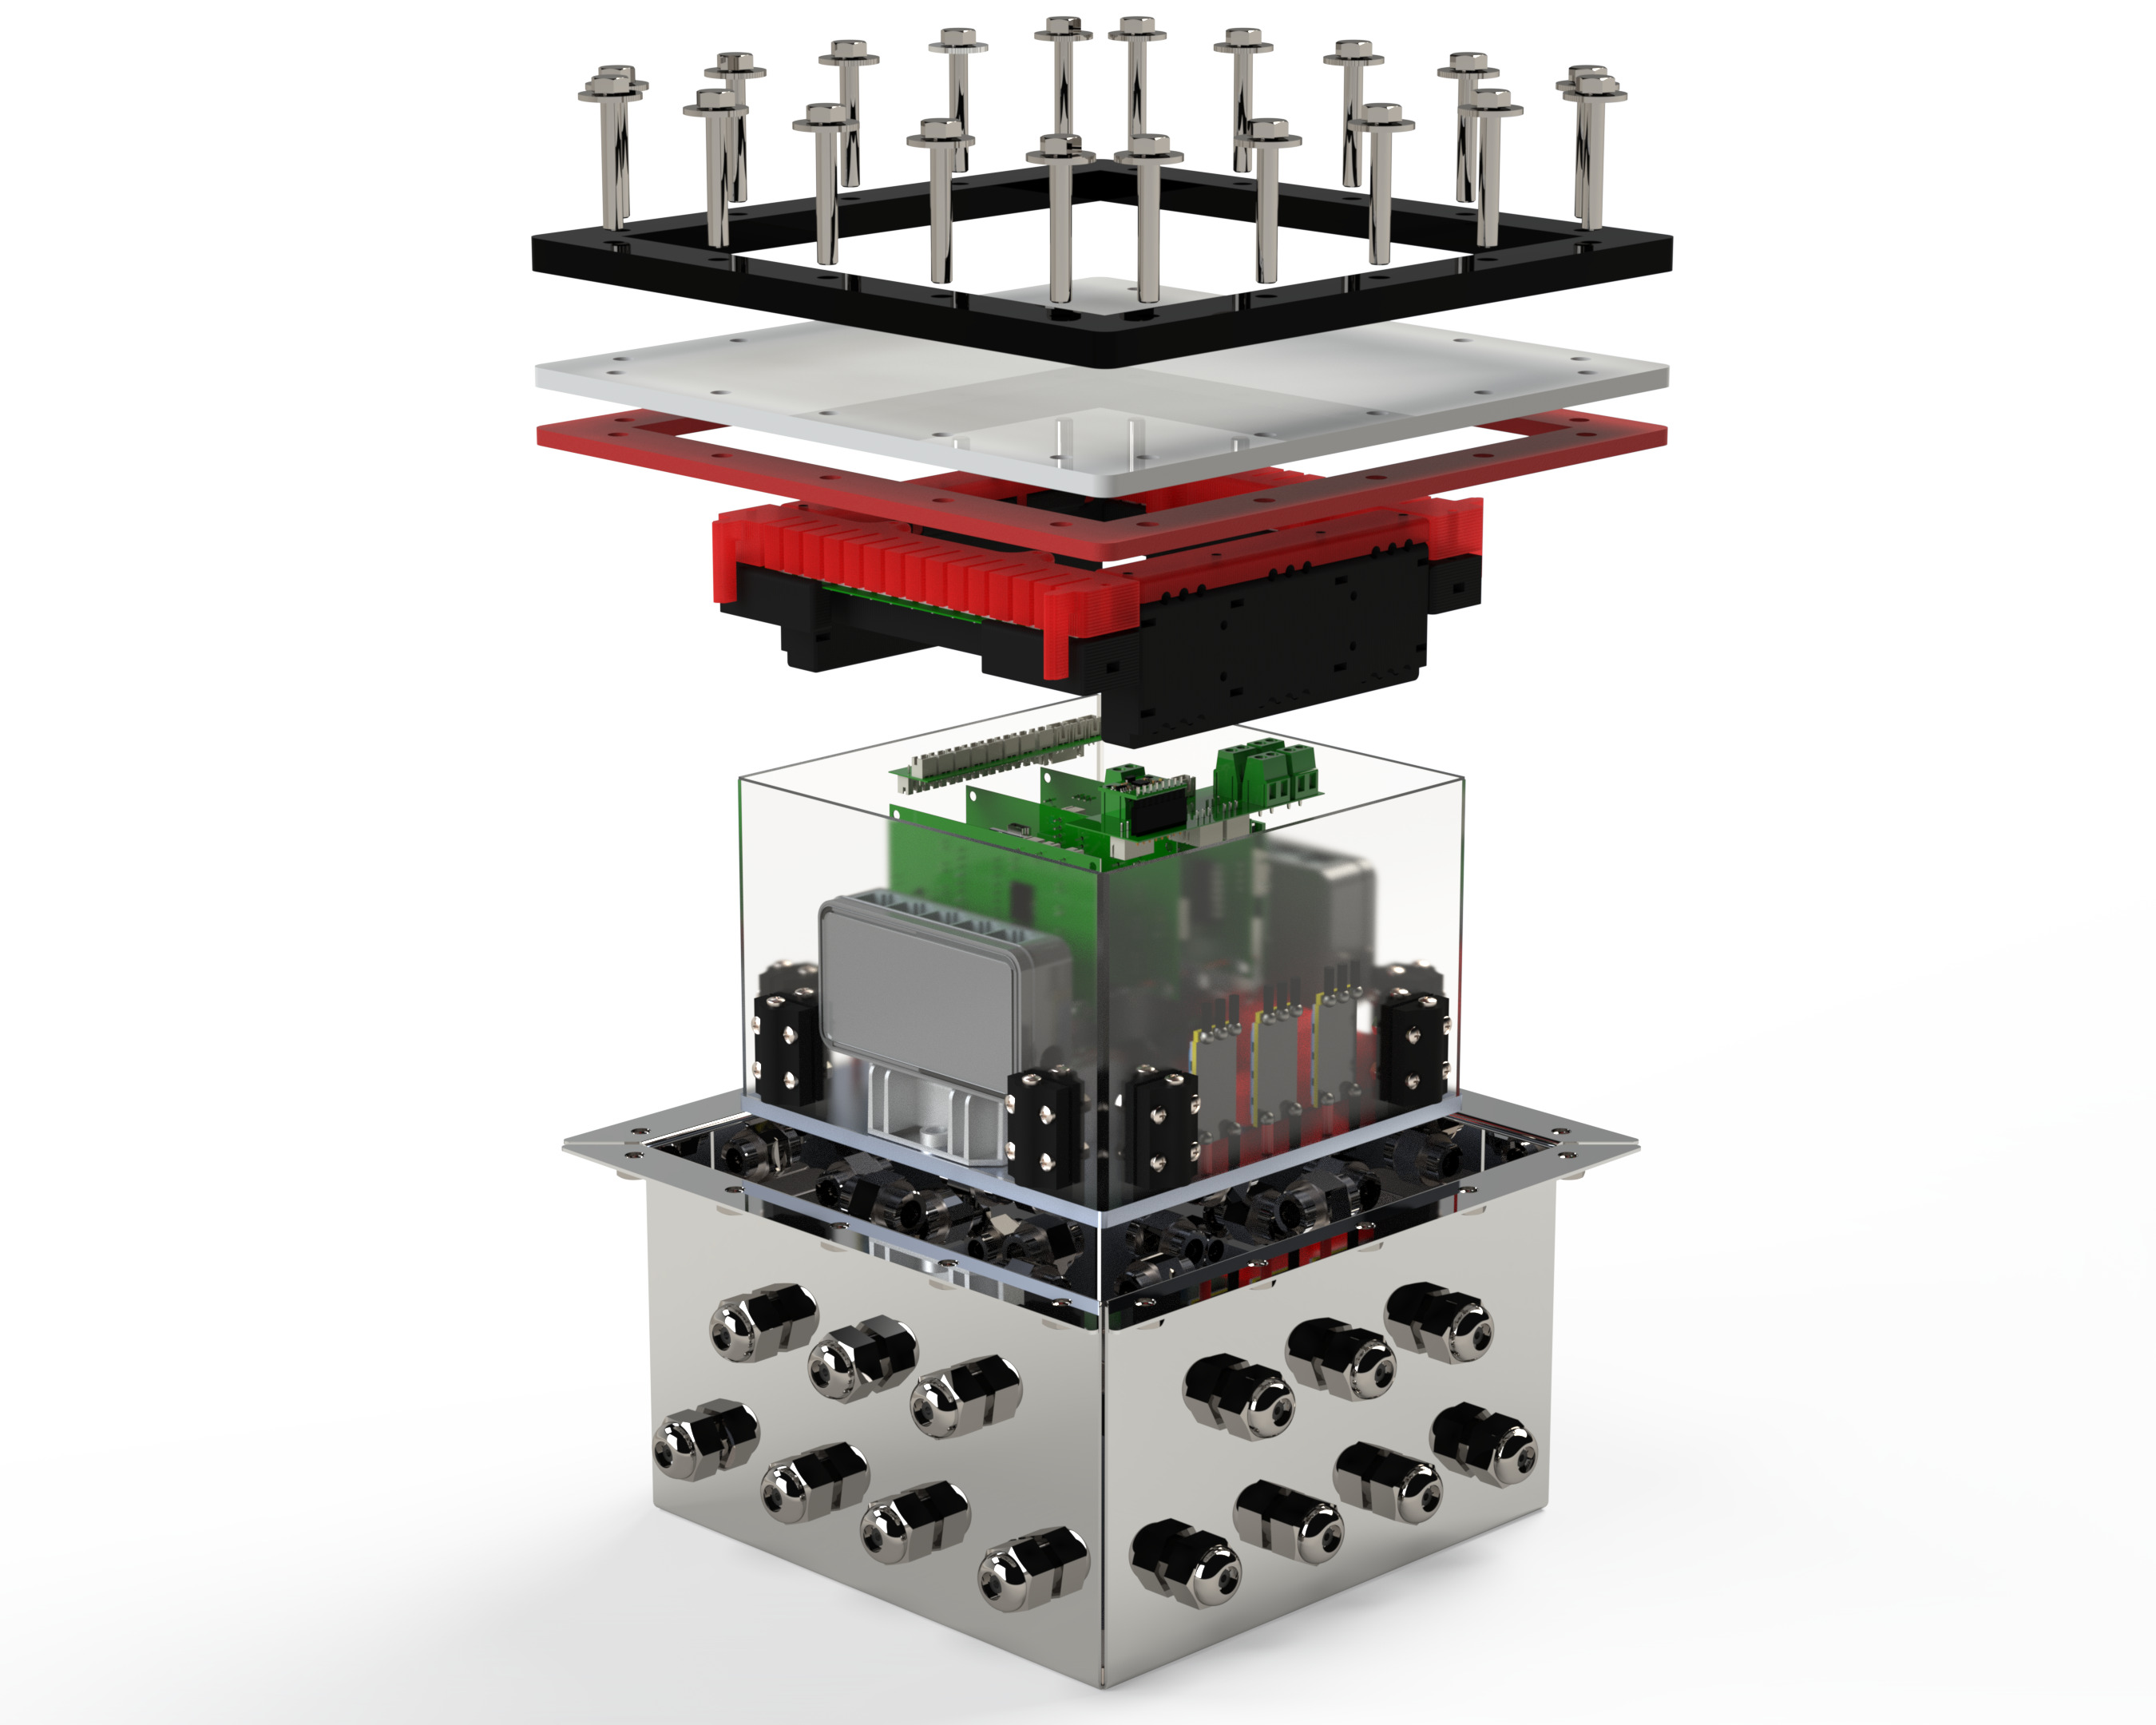
\includegraphics[width = 0.4\textwidth,height= .2\textheight]{box23 (10)_Camera_SOLIDWORKS Viewport}
	\caption{Polaris Box.}
\end{wrapfigure}
\textcolor{orange!60}{
\subsubsection{2- Electronics Box}}	
In the last 2 years, the electronics housing took a cylindrical shape and was made of HDPE, which resulted in the irregularity of the ROV’s weight and the waste of materials, which cost us loads of  money. This year we decided to go by a different approach, which was to use a cubic stainless-steel box, which was lighter and sturdier than HDPE housings. A comparison was made between choosing stainless-steel or Aluminum, but we decided to go with stainless-steel due to its high strength which would allow us to use a thinner sheet. Moreover, it will help dissipate the heat from the internal electronics to the surrounding water.\\
\begin{wrapfigure}{r}{.4\textwidth}
\centering
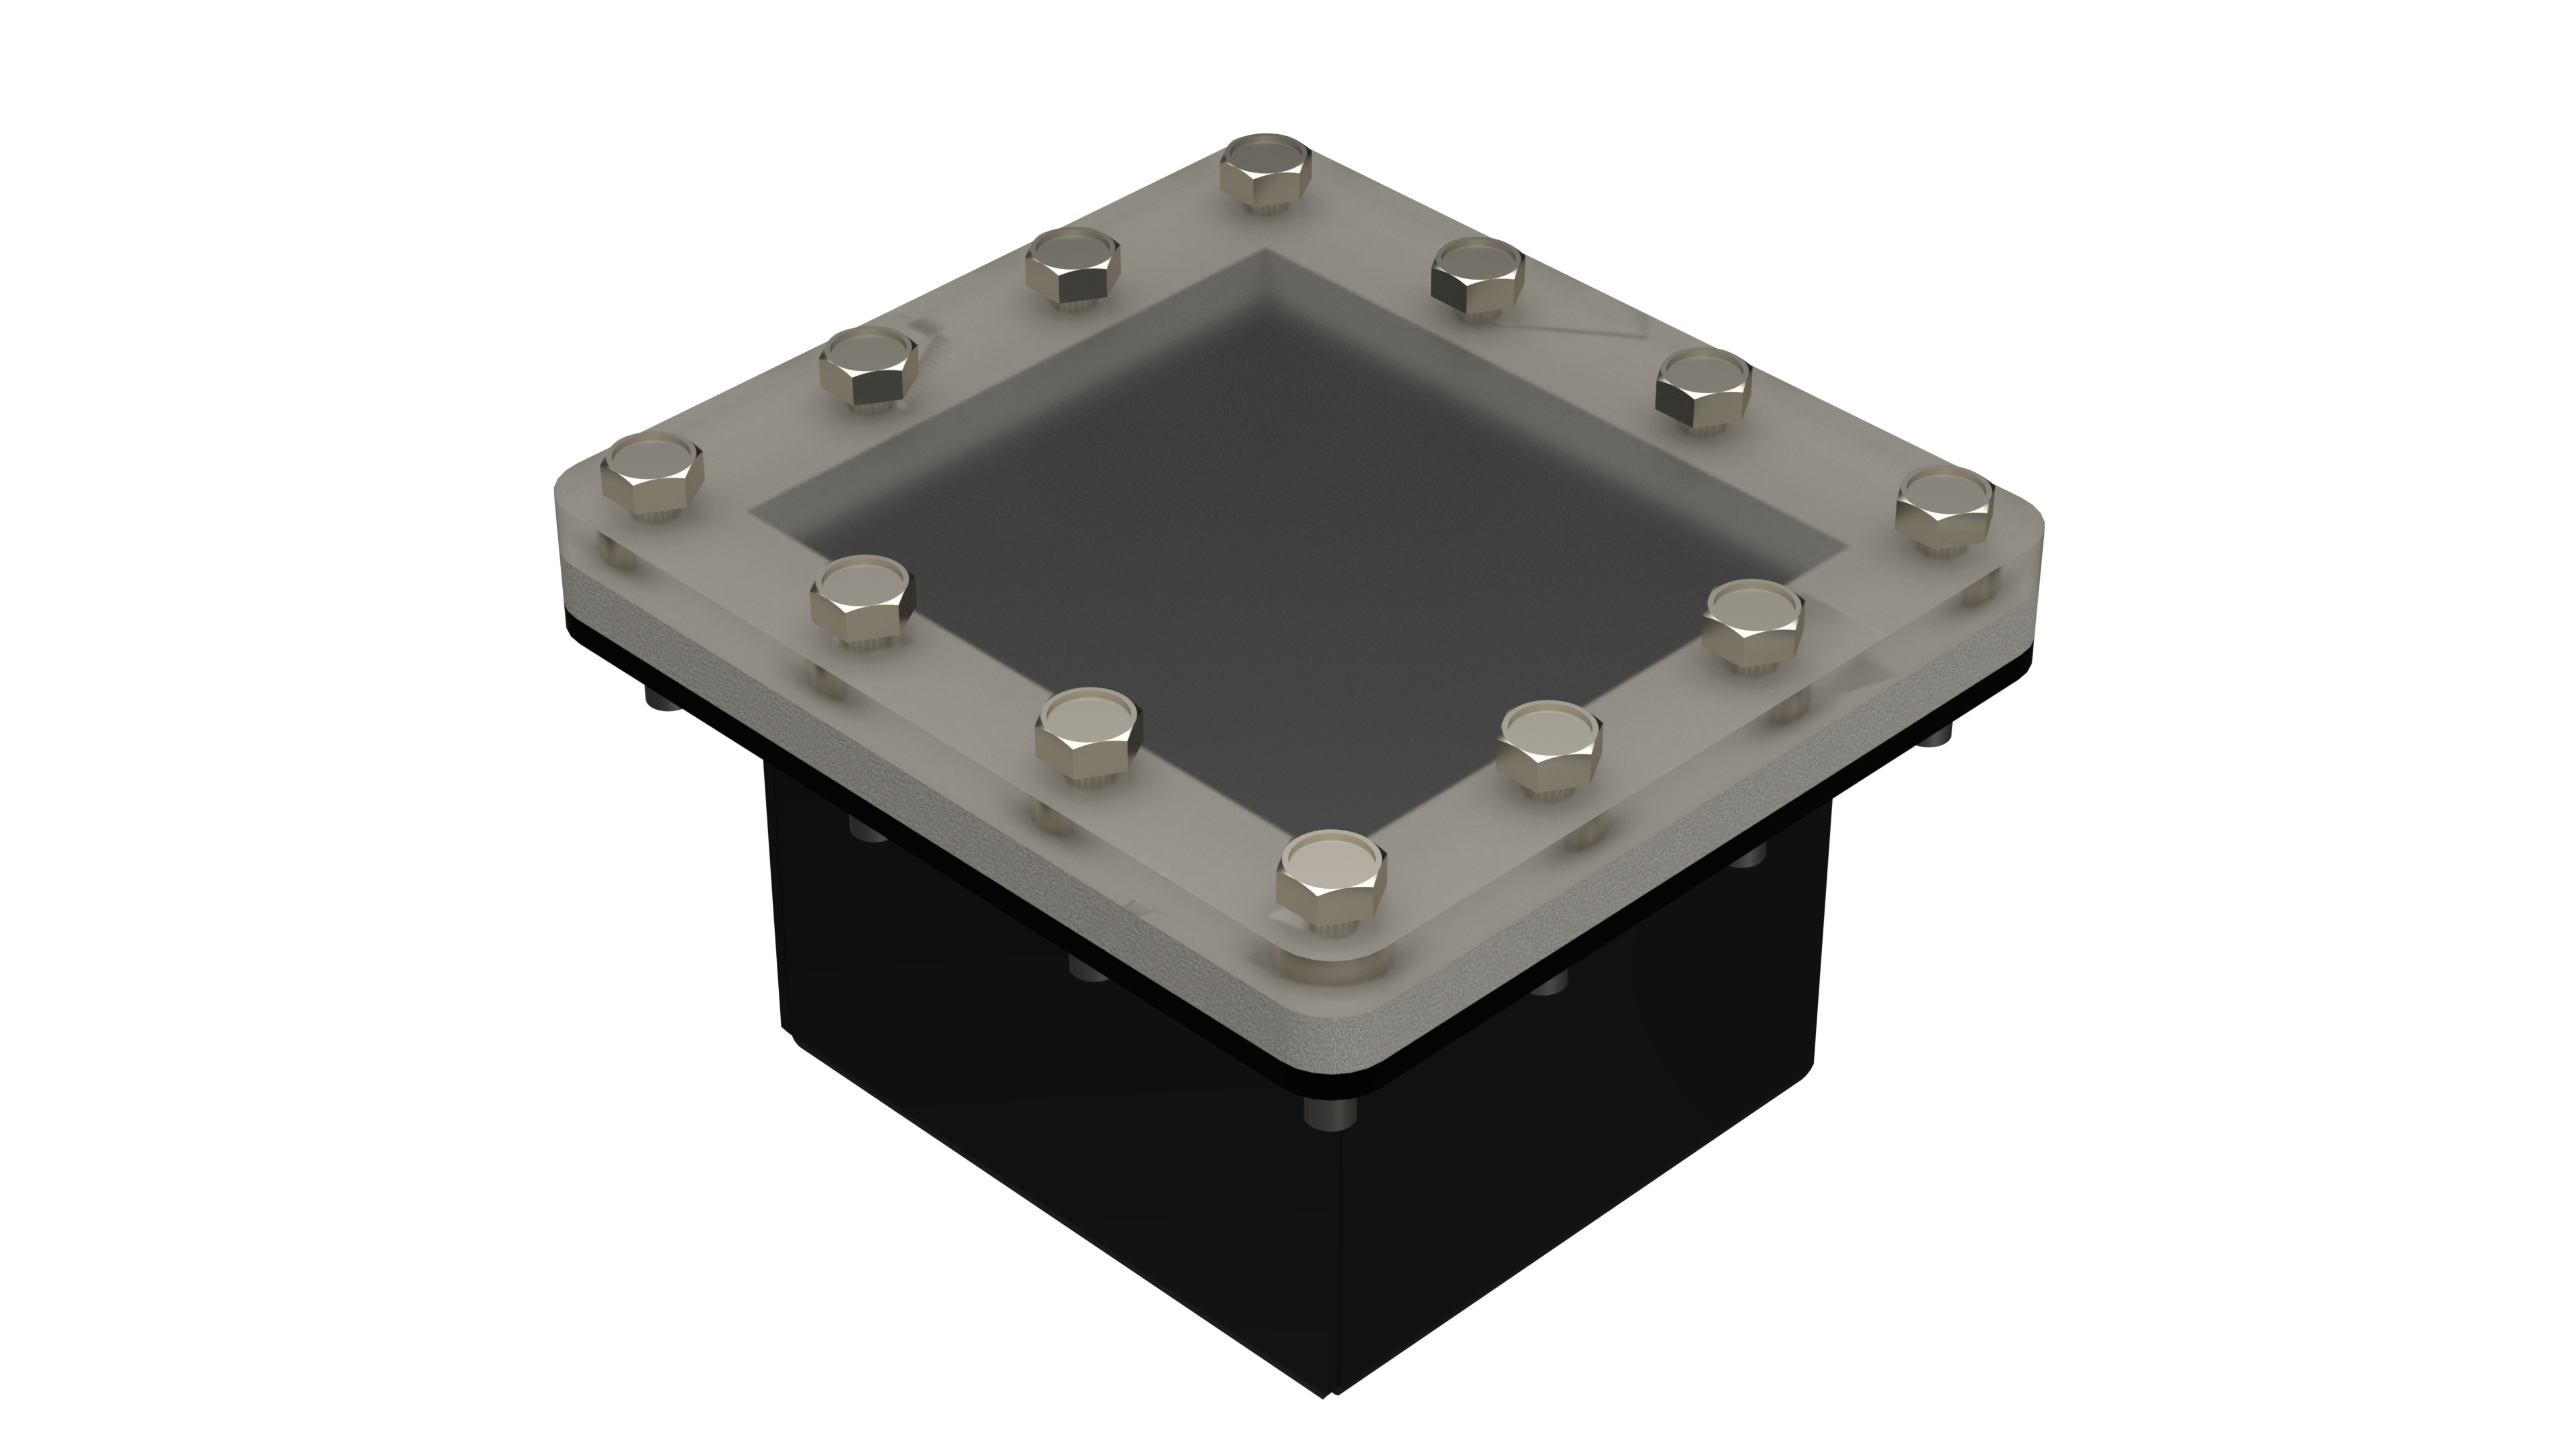
\includegraphics[width=0.4\textwidth,height= .105\textheight]{Untitled Project_Camera_Default Camera}
	\caption{Polaris Camera.}
\end{wrapfigure}

\textcolor{orange!60}{
\subsubsection{3- Camera}}
We wanted to provide clear vision for our pilot and eliminate blind  spots as much as possible, so we modified camera fixations to  achieve that purpose.
\\

\textcolor{orange!60}{
\subsubsection{4- Thrusters and Propulsion System }}
Our RND unit has been making major accomplishments concerning the  propulsion system. Since 2021 we have used T200 from Blue Robotics,  which have provided us with adequate thrust force. We are currently  working on manufacturing our own thrusters, using waterproofed DC  brush-less motors and 3d printed thyroidal propellers. 
This year, our goal was to design a propulsion system with the highest  
efficiency and the lowest possible cost, so we reused the T200 thrusters we had from previous years. The parts were damaged and needed proper maintenance before being integrated into our ROV.
Regarding the positioning and configuration of the thrusters, we agreed on using 6 thrusters, and to achieve stable vector drive, the propulsion system was configured in a way such that two thrusters are used to move the ROV in its vertical plane. Four other thrusters are used to move the ROV in the horizontal plane. 
Each of the four horizontal thrusters is fixed such that its center axis  of rotation is placed with an inclination of a value of 60°/30° relative  to the surge direction of the ROV in the horizontal plane. This  configuration allowed all thrusters to contribute to the total propulsion in 5 cardinal directions (surge, sway, heave, yaw, and pitch), gave  priority (in terms of speed) to forward and backward motion, and  minimized flow interference with the electronics housings in the  center of the vehicle.For the safety of personnel and equipment, thrusters guards are mounted on both sides of the  thrusters’ core nozzles to prevent foreign objects from entering the thrusters. \\
\textcolor{blue!40}{
\subsubsection{D- Computational Fluid Dynamics}}
Drag refers to the resistance encountered by an object as it moves  through a fluid medium, such as water. By accurately calculating drag  forces, we managed to optimize the performance of our ROV. 
We visualized the shape of artery vertices, and accordingly, the main  components of Polaris were modified to obtain the lowest drag  coefficient, and all this was done by conducting CFD analysis using  ANSYS Fluent. The final design is shown in the figures, where we visualized pressure contours, velocity contours, and streamlines. The  final drag coefficient was 0.9 as printed from the Fluent drag force and  coefficients report.\\
\textcolor{blue!40}{
\subsubsection{F- Buoyancy}}
Achieving good stability configuration and smooth suspension of our ROV underwater has  always been one of the goals for our mechanical team. Also, for safety purposes, it was  decided to make the ROV slightly positively buoyant. To achieve these goals, we started by  locating the center of buoyancy (CB) relative to the center of gravity (CG) with the help of CAD  software (Solid Works), we intended to put bigger weights at the lower base and floating  material at the higher base to increase the distance between (CB) and (CG) which provided better stability for the whole system. At the end, mechanisms were mounted on Polaris’ frame,  and the result was that Polaris was negatively buoyant by 1.25 Kg, so we decided to put rigid  Polyurethane (Foam) with a density of 36 Kg/m3. On calculating the required volume, we  decided to put cylindrical foam around the electronics housing. \\
\textcolor{blue!40}{
\subsubsection{G- Wire Selling}}
We tried many methods for wire sealing, however we decided to use cable glands to pass cables through safely easily and guarantee maximum sealing against water infiltration.
\vspace{3cm}
\textcolor{blue!90}{
\subsection{Electrical System}}
\begin{wrapfigure}{r}{.36\textwidth}
\centering
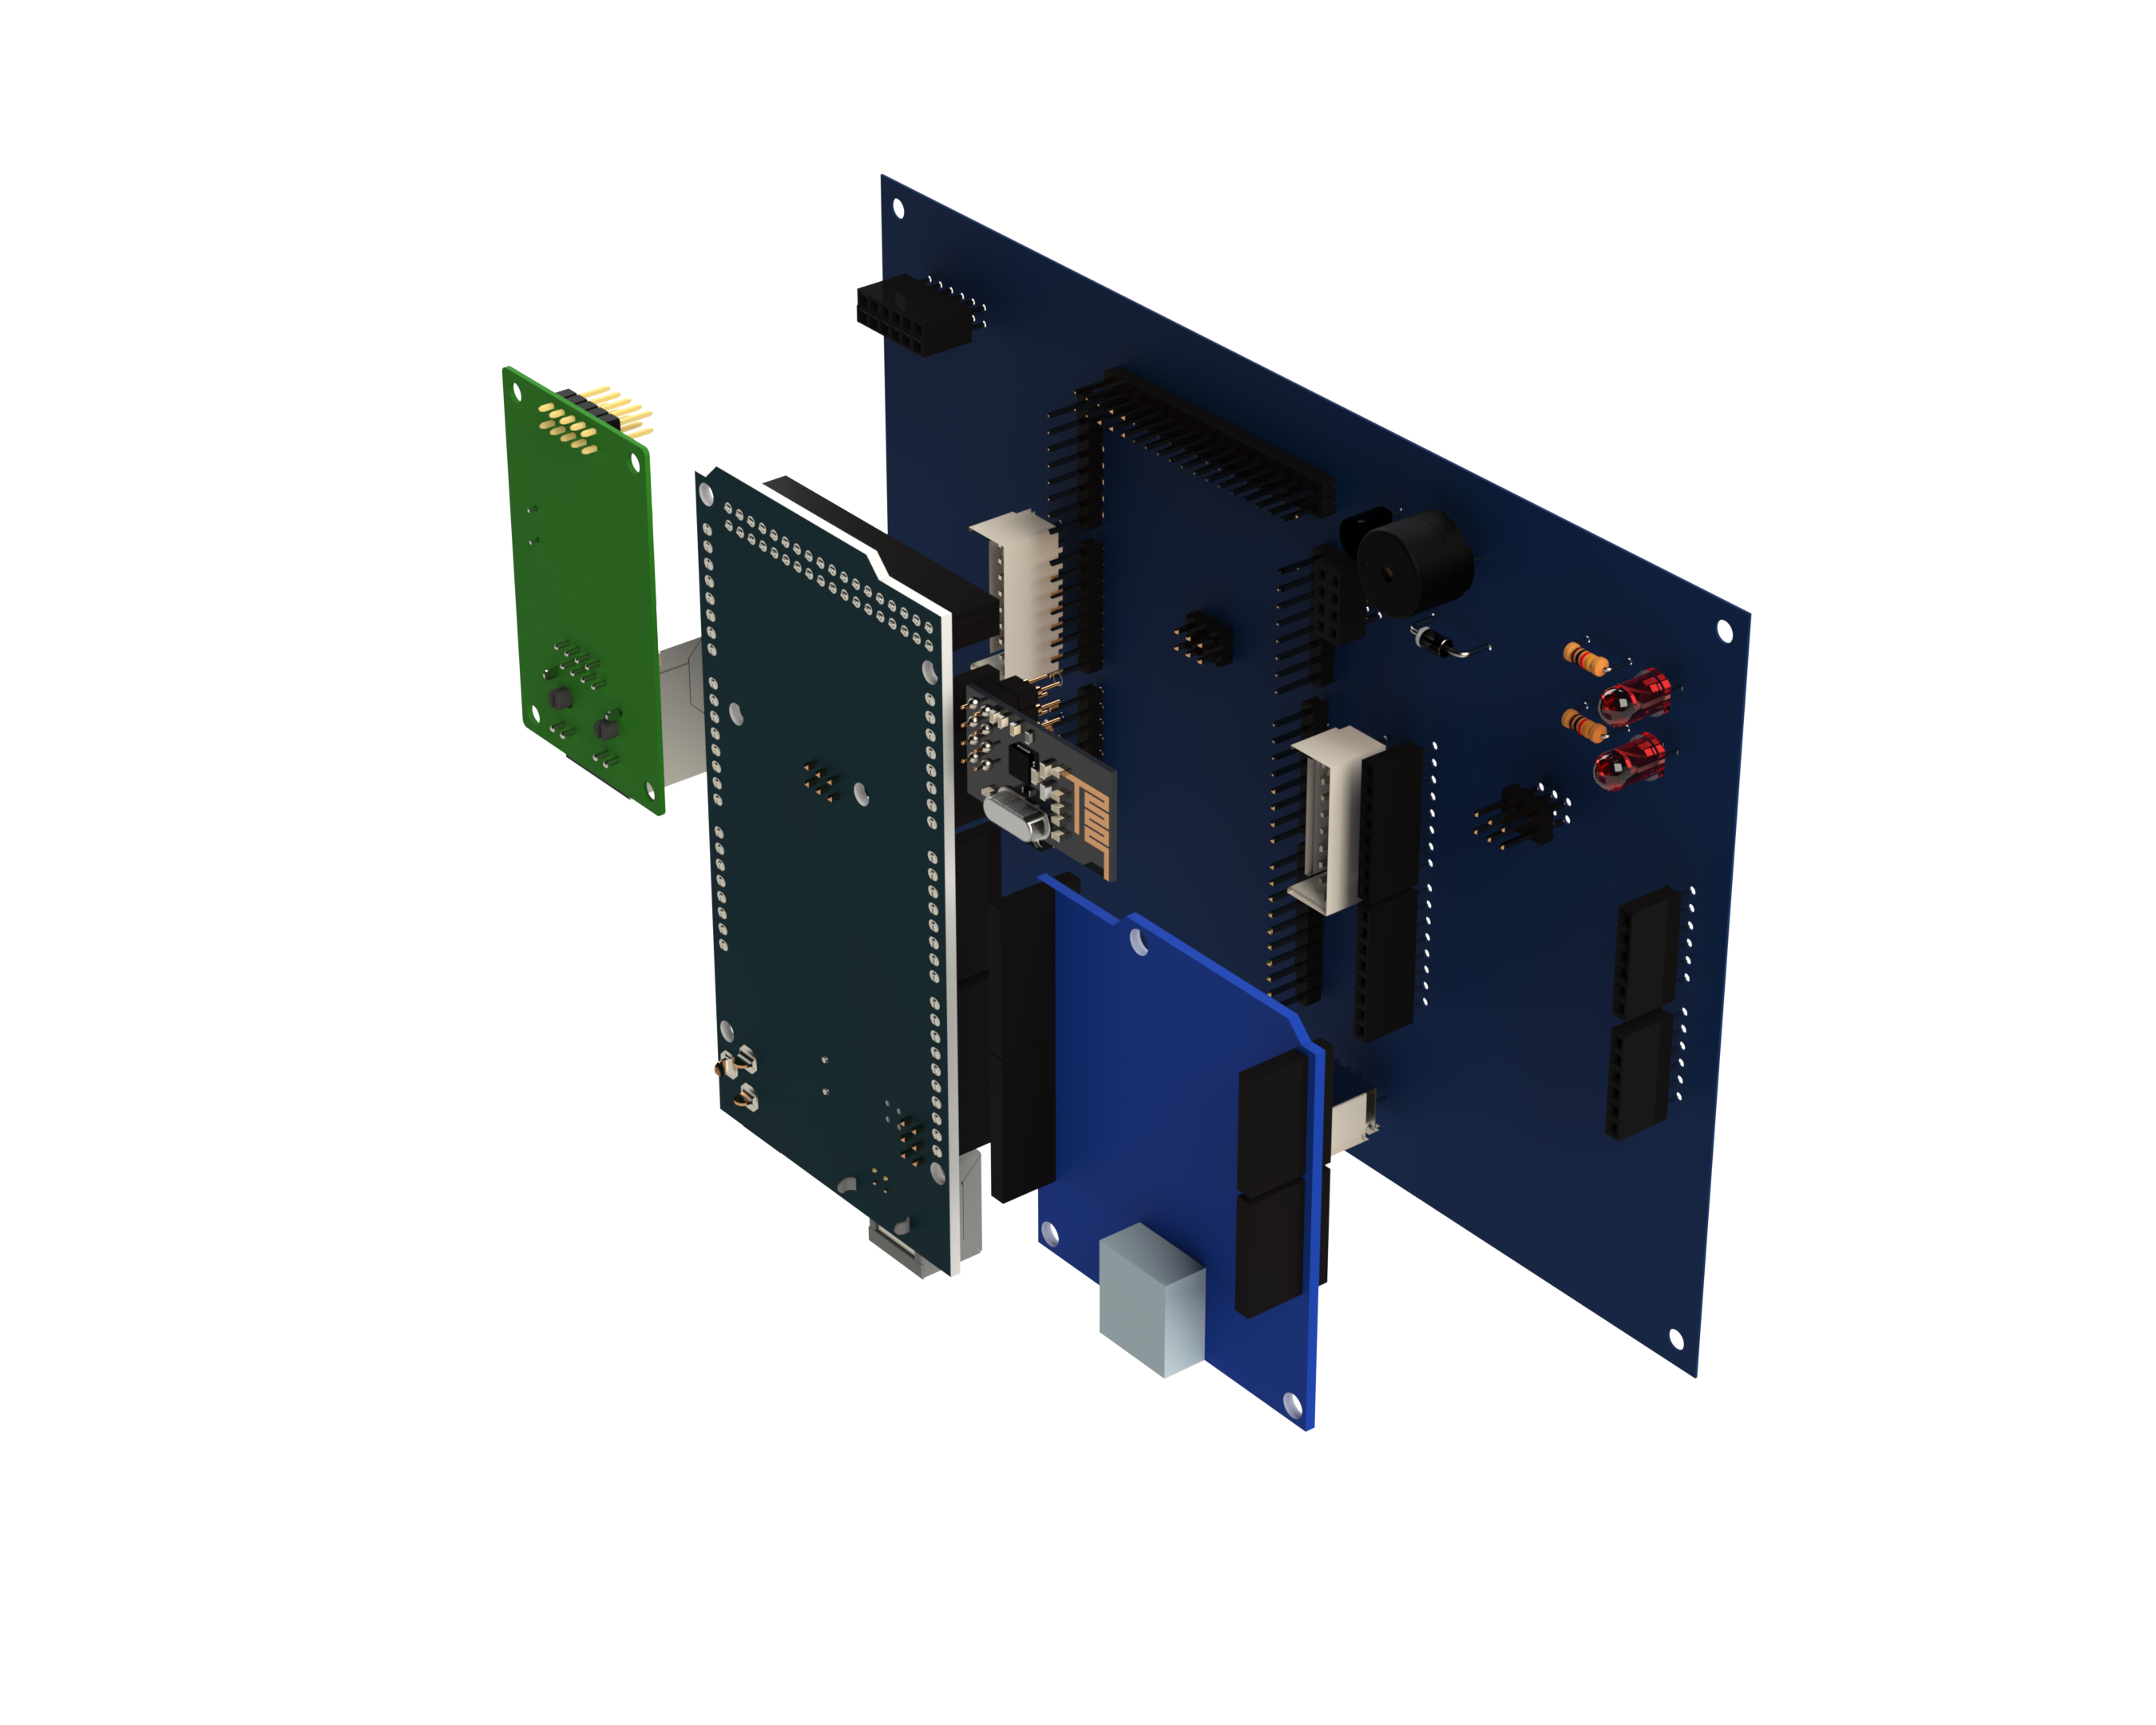
\includegraphics[width=.36\textwidth,height= .2\textheight]{console board (5)}
\caption{Polaris Console Board.}
\end{wrapfigure}
\textcolor{blue!40}{
\subsubsection{A- TCU(Tether Control Unit)}}
The biggest advantage about our TCU is its plug and play feature,  where you only need to power it up and you’re good to go in no time. 
To connect the TCU to the ROV through the tether, polarized  connectors are used. For the power connection, the XT-60 connector  is used, due to its firmness and being polarized, avoiding any miss wiring during setup. In addition, wire terminals are covered with heat shrinks avoid unexpected shorts in the TCU. For communication, a  single RJ-45 Ethernet connector is used since it provides a firm and  stable connection. 

\textcolor{orange!90}{
\subsubsection{1- Main Controller}}
As for controlling Polaris from the TCU, we’ve decided to reuse our PS3 connectors. 
game pad since it has enough buttons that satisfy our needs. The game pad is connected to Arduino Mega -the micro controller we use  topside- via a USB host shield. The micro controller reads the game pad’s readings, applies a vector algorithm, and then sends the required  thrusters’ direction and speed to the ROV.\\
\textcolor{orange!90}{
\subsubsection{2- GUI (Graphical User Interface) }}
GUI is a vital tool for the co-pilot so they can monitor Polaris’ status and view feedback from the used sensors so that they are always  aware of any problem before it is too late. This is why we made sure  our GUI is not at the risk of crashing or malfunctioning and chose  PyQt5 to implement the interface. For additional ease of use, each  task is separated into its own tab so that the co-pilot would not be  distracted while performing a specific task. 
\\
\textcolor{blue!40}{
\subsubsection{B- Tether}}
We incorporated a CAT6 Ethernet cable in the communication between the box and the TCU by connecting it to a network switch to communicate with the Ethernet module connected to our TCU micro controller. We preferred the CAT6 type over CAT5e because of the greater transmission performance and better immunity from external noise. CAT6 is also more malleable and can handle harsh conditions. We also covered the tether with a Tec flex cover to maintain cable management and provide the tether with more  protection As for the power tether, we decided to go with a 13 WG stranded cable as this gauge can  stand the rated current draw, while also having the least voltage drop and smallest cross sectional area (which meant the least affected by drag) among all other options.
The tether also includes a pneumatic cable to supply air to all pneumatic contraptions mounted  on the ROV. \\
\textcolor{blue!40}{
\subsubsection{C- Electronics}}
\textcolor{orange!90}{
	\subsubsection{1- Power Conversion }}
This year, we utilized seven DC-DC converters to step down 48VDC to 12VDC, four of which can draw a maximum current of 30A, and two others can stand a maximum of 20A. They are  used to power our thrusters. The seventh, with a 5A maximum current, is used for powering our  control circuit, six cameras, lights, and solenoids. This configuration was proposed to solve 2  major problems that had occurred in the previous years which are the camera feed lag and  communication distortion due to the transient effect of thrusters when the cameras and electrical  unit were connected to the same converter, but this year we decided to use the seventh as mentioned before. This made the power distribution more efficient and better distributed than  before.\\
\textcolor{orange!90}{
	\subsubsection{2- Electronics Box System}}
This year, our focus for the electrical system was the ease of maintenance  
and modularity, as well as decreasing the size as much as possible so as not to cram the electrical housing. Our system mainly consists of one double layer control board. Polaris’ control board is centered around an ESP32 as it offers many features, such as its small size (compared to other micro controllers offering the same number of pins), built in Wi-Fi (that enables communication and integration with other devices and networks), and its high performance.
One challenge that arises when working with ESP32 is the limitation of  the pins, but by using a shift register, we were able to expand the number  of pins available for connecting different components to our control board. 
For the thrusters’ operation, we decided to use ESC motor drivers to  control the internal brush less DC motors. We chose to buy it over making  our own for many reasons, such as the small size, better efficiency, the  lack of need for a heat sink, and it has current protection. Also, a bullet  connector is used to connect the ESC with the thrusters to be easily  detached and pass through the glands and separate the thrusters from  the system for troubleshooting and debugging.
At the end, we were able to integrate our system into a single control  board that includes sensors, actuators, the micro-controller, and all its  peripherals, eliminating the need to divide the system into several boards  of different functions such as before. \\
\textcolor{orange!90}{
	\subsubsection{3- Electronics Box Components }}
\textcolor{red!90}{
	\subsubsection{I- Sensors}}	
To keep the motion of the ROV smooth and stable as much as possible,  we used two different types of sensors.\\
\\

\textcolor{green!90}{
	\subsubsection{IMU}}	
The MPU6050 IMU (6 Degrees of Freedom) has both a 3-axes  accelerometer (which measures acceleration) and 3-axes gyroscope  (which measures angular velocity) integrated on a single chip. The  previously mentioned data is enough to calculate all 3 angles of rotation,  roll, pitch and yaw, so that we can control Polaris‘ orientation and position. \\
\textcolor{green!90}{
	\subsubsection{Pressure Sensor}}	
The MS5540C pressure sensor was used to calculate Polaris’ depth underwater. The sensor measures the pressure, then by using the relation, we can calculate the depth of the ROV.\\
\textcolor{blue!40}{
	\subsubsection{D- Communication}}
\textcolor{orange!90}{
	\subsubsection{1- Top Side }}	
As for the communication between the TCU and Polaris, Ethernet UDP “User  Data gram Protocol” was used. The communication is full duplex; hence  Polaris can send and receive data simultaneously. ENC28J60 Ethernet  controller was chosen to serve as an ethernet network interface for the used   
micro controllers since they are equipped with SPI “Serial Peripheral  Interface”. On top of that, the “Ethernet” library was used to control.\\
\textcolor{orange!90}{
	\subsubsection{1- Underwater Side }}	
This year, we decided to use an ESP32 micro controller instead of using three Arduino Nano.  This reduced the error due to communication between the three Arduino Nanos. The ESP32  offered several advantages over the Arduino such as its higher processing power, its dual core architecture which allowed us to multitask and its built-in Wi-Fi which allowed us to upload  different codes on Polaris’ ESP32 wireless.\\
\textcolor{blue!40}{
	\subsubsection{E- Vision System}}
\textcolor{orange!90}{
\subsubsection{Camera Control}}	
We have used a camera module that is made to operate and receive feeds from the cameras on the ROV. It can capture and process video feeds from various types of cameras. Moreover, it can be configured to work with either an external or local camera, depending on the specific requirements of the task. The module also provides advanced features for managing video streams, such as handling lost connections and automatically  reconnecting to the camera when required. \\
\\ 
\\
\textcolor{blue!90}{
\subsection{Mission Tools}}
\textcolor{blue!40}{
\subsubsection{A- Mechanical Mission Tools}}
\begin{wrapfigure}{l}{.3\textwidth}
	\centering
	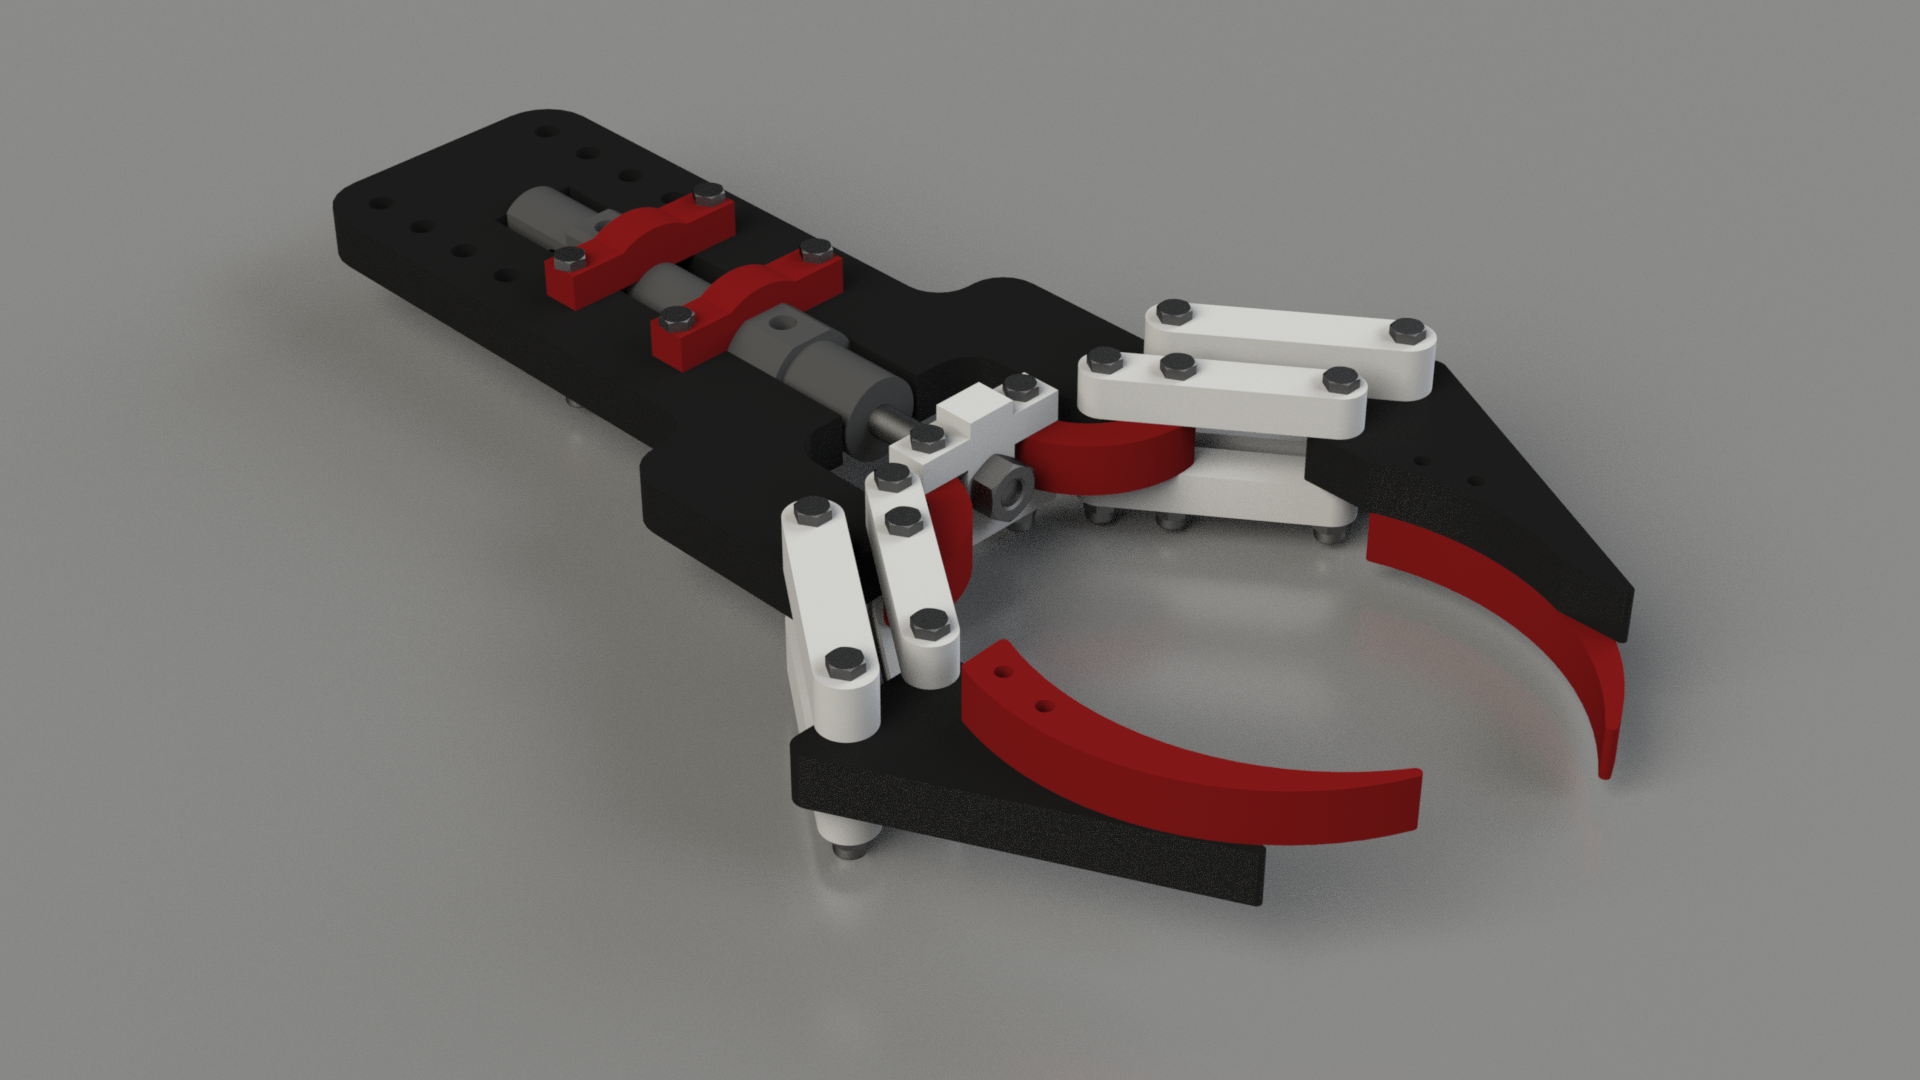
\includegraphics[width = .3\textwidth, height=.15\textheight]{micop7}
	\caption{Polaris Manipulator.}
\end{wrapfigure}
\textcolor{orange!90}{
	\subsubsection{I- Multi functional Manipulator }}	
As per the competition’s requirements, we built a lightweight  manipulator that gives us two degrees of freedom and can execute  underwater tasks efficiently. 
To achieve a high gripping force, it is pneumatically actuated with a  32*25 mm cylindrical piston. We modified its end effector to provide a  large contact area, so that it can hold up objects up to 120mm in  diameter. Moreover, it was designed to deal with various cross manipulator.    sectioned shapes, and rubber was added to provide high friction with objects. The gripper is made of high-density polyethylene (HDPE) due to its high durability and easy mach inability as  it was cut on a CNC laser cutting machine.\\ 
\textcolor{blue!40}{
\subsubsection{B- Image Processing Tools}}	
\textcolor{orange!90}{
\subsubsection{I- Measuring the Length of Fishes}}
In order to measure the length of fishes model ,our Team create a GUI to make it more easy and professional, in this GUI we can insert the pictures, the model will work and write the length we want to know the category of it, and the model will select all fishes with this length, we can also get the all fishes’ length by display all icon in our GUI. \\
\textcolor{orange!90}{
\subsubsection{II- Monitor the Lake Against Pollution }}	
To identify shapes (or pollutants) on the ground, we grab a frame of the sheet of paper from our camera feed through our GUI and run multiple image processing operations on this frame. We start by obtaining contours to isolate the black shapes on the paper then in order to differentiate between multiple shapes (squares, crosses, etc.) we used a process that reduces each contour  into a collection of corner points. From that we can deduce what shape each contour represents and thus carry out our final calculation.\\ 
\textcolor{blue!90}{
\section{Safety Rational}}
\textcolor{blue!40}{
\subsubsection{A- Design Safety and Philosophy}}
Safety is our top priority in Torpedo we aim towards keeping our engineers safe, protected, and satisfied to achieve high-quality work progress. We keep safety aspects for designing, manufacturing, testing, and maintaining our ROV for all tasks. We follow all safety protocol points, and safety checklists and work in a safe work environment so  that we keep our members safe. 

\textcolor{blue!40}{
	\subsubsection{B- Members’ Safety}}
All members must wear personal protective equipment (PPE) such as gloves, goggles, and face  masks while machining or working with epoxy or fibers to prevent the inhalation of dangerous  chemicals or particulates. Cords are kept out of aisles and walkways to keep the area neat and  prevent tripping. Also, a safety-aid kit is always present in our workshop in case of any accidents.  
\begin{table}[H]
\centering
\caption{Equipment and Operational Safety}
\begin{tabular}{|p{8cm}|p{8cm}|}
\hline
\textcolor{red!80}{Mechanical}&\textcolor{red!80}{Electrical}\\ \hline
Never work alone in the workshop. & All electrical equipment has been  enclosed in sealed housing. \\ \hline
Make sure your work piece is fixed  securely before work.  & All hardware circuits are connected  to fuses according to the maximum  load. \\ \hline
Do not talk to anyone operating  electrical equipment machinery,  e.g., Circular saw. &
Our TCU is equipped with an  emergency switch, in case of any  urgent situation.  \\ \hline
Inspect equipment before use. & Our tether is covered with a braided  sleeve to protect the tether. \\ \hline
Wear gloves and goggles when  working with a drill and cutting tools. &  Cables and wires must be isolated.\\ \hline
Use cap nuts to cover bolts. & Wear gloves and goggles while  dealing with soldering irons. \\ \hline
All sharp edges must be filleted. & \\ \hline
\end{tabular}
\end{table}

\begin{table}[H]
	\centering
	\caption{Safety Checklist}
	\begin{tabular}{|p{8cm}|p{8cm}|}
		\hline
		\textcolor{red!80}{Offshore Safety}&\textcolor{red!80}{Underwater-Before Mission  Safety}\\ \hline
The ROV is transported to the  competition playground covered in  bubble wrap to protect it against  impact.  & Make sure the electric box is not  leaking (no detecting leakage data  from leakage sensors, and no  bubbles are going up). \\ \hline		
Nuts are well-tightened. Thrusters  are free from obstructions. & Perform a short wet test to make  sure all manipulators and thrusters  are fully functional. Test the main  gripper to make sure the air  compressor is properly connected  and functioning. \\ \hline
The tether is well connected to the ROV and the TCU. & Make sure the cameras’ signals are not distorted.\\ \hline
Check the strain relief of the tether.  & Check the converters’ current to ensure your system is working with  no danger. \\ \hline
The Area is clear and safe for the tether man motion. & \\ \hline
Dry start-up to make sure of the penetrability of the ROV. & \\ \hline
	\end{tabular}
\end{table}

\begin{table}[H]
	\centering
	\caption{Safety Checklist}
	\begin{tabular}{|p{8cm}|p{8cm}|}
	\hline
\textcolor{red!80}{Underwater-During Mission Safety}&\textcolor{red!80}{After Mission Safety}\\ \hline
Make sure the tether does not  surround the ROV so that it would not be damaged and verify the tether  is free of kinks. ‘Tether man job’. &Lift the ROV out of the water. \\ \hline
The main power is turned off, and the ROV is lifted out of the water in case of leakage. & Turn off the main power supply. \\ \hline
& Turn off the air compressor. \\ \hline
&Cover the ROV in bubble wrap to transport it back to the Torpedo workshop. \\ \hline
	\end{tabular}
\end{table}
\textcolor{blue!90}{
	\section{Conclusion}}
\textcolor{blue!40}{
	\subsubsection{A- Technical Challenges}}
\textcolor{orange!90}{
\subsubsection{1- Mechanical Challenges}}
Our mechanical team faced a lot of challenges this year, including designing the ROV from  scratch to be light, have low drag force, and have additional space for mission tools to be mounted to prevent the previous years’ problems. When it comes to fabrication, lots of ideas  were discussed about the material of each component, including their pros and cons then  materials were chosen to provide high efficiency while being cost-effective. However, to ensure  the electrical components' safety, a lot of sealing techniques were tested, and we chose the best  one of them. Moreover, this year’s tasks represented the most difficult challenge for us. We  spent a lot of time searching for and designing and developing mission tools to meet the task  requirements.\\ 
\textcolor{orange!90}{
	\subsubsection{2- Electrical Challenges}}
This year we faced multiple challenges in our system, one of which was that we wanted to  integrate all our system in one board, housing the ESP32 as its micro controller. The ESP32,  however, has a limited number of pins which were not enough for the devices in our electrical  system. As a solution, we used a shift register as an IO expanded so that the ESP32 can interface  with more devices through the same number of pins. Another problem was the lack of resources for the ESP3 platform unlike other alternatives (such as the Arduino). To solve this problem, we had to hack into the available libraries to make them compatible with the ESP32, which was a  part of our RnD plan.\\
\textcolor{blue!40}{
	\subsubsection{B- Non-Technical Challenges}}
The biggest challenge we faced this season was changing and improving the configuration of the non-technical techniques we used in making our report, and non-technical documents. We were able to handle this problem by including the whole team in the process, where the  mechanical and electrical teams worked together to improve our team on all technical and non-technical sides, with the help of the old members, mentors, and seniors which gave us a lot of  advantages to organize our schedules. \\
\textcolor{blue!40}{
\subsubsection{C- Technical Lessons Learned}}
This year, one of our main goals was to avoid the obstacles we had experienced previously, be  it the problems in our old vehicles or our way of managing things in general. This made us approach problems differently and find perfect solutions for them. Also, to acquire a more  stable system throughout the year, the team had been working with many programming  languages such as Python and C++, as well as enhancing our ability to design and simulate  stresses and flow using Solid Works®, ANSYS® and Fusion 360®. 
We have also followed new techniques in making system design for our ROV, and we have dealt  with new components with new techniques which helped our team members increase their  technical knowledge and go through new experiences. \\
\textcolor{blue!40}{
	\subsubsection{D- Future Improvements }}
1- Doing research into new micro controllers and whether they would be better for our use  case or not. \\
2-Improve our communication system and make it more reliable and efficient. \\
3- Use reliable waterproof plugs for faster maintenance and replacement. \\
4- Design new modular and adjustable mission tools. \\
5- Look into new motion and control systems to achieve better maneuverability. 
\begin{wrapfigure}{r}{.3\textwidth}
	\centering
	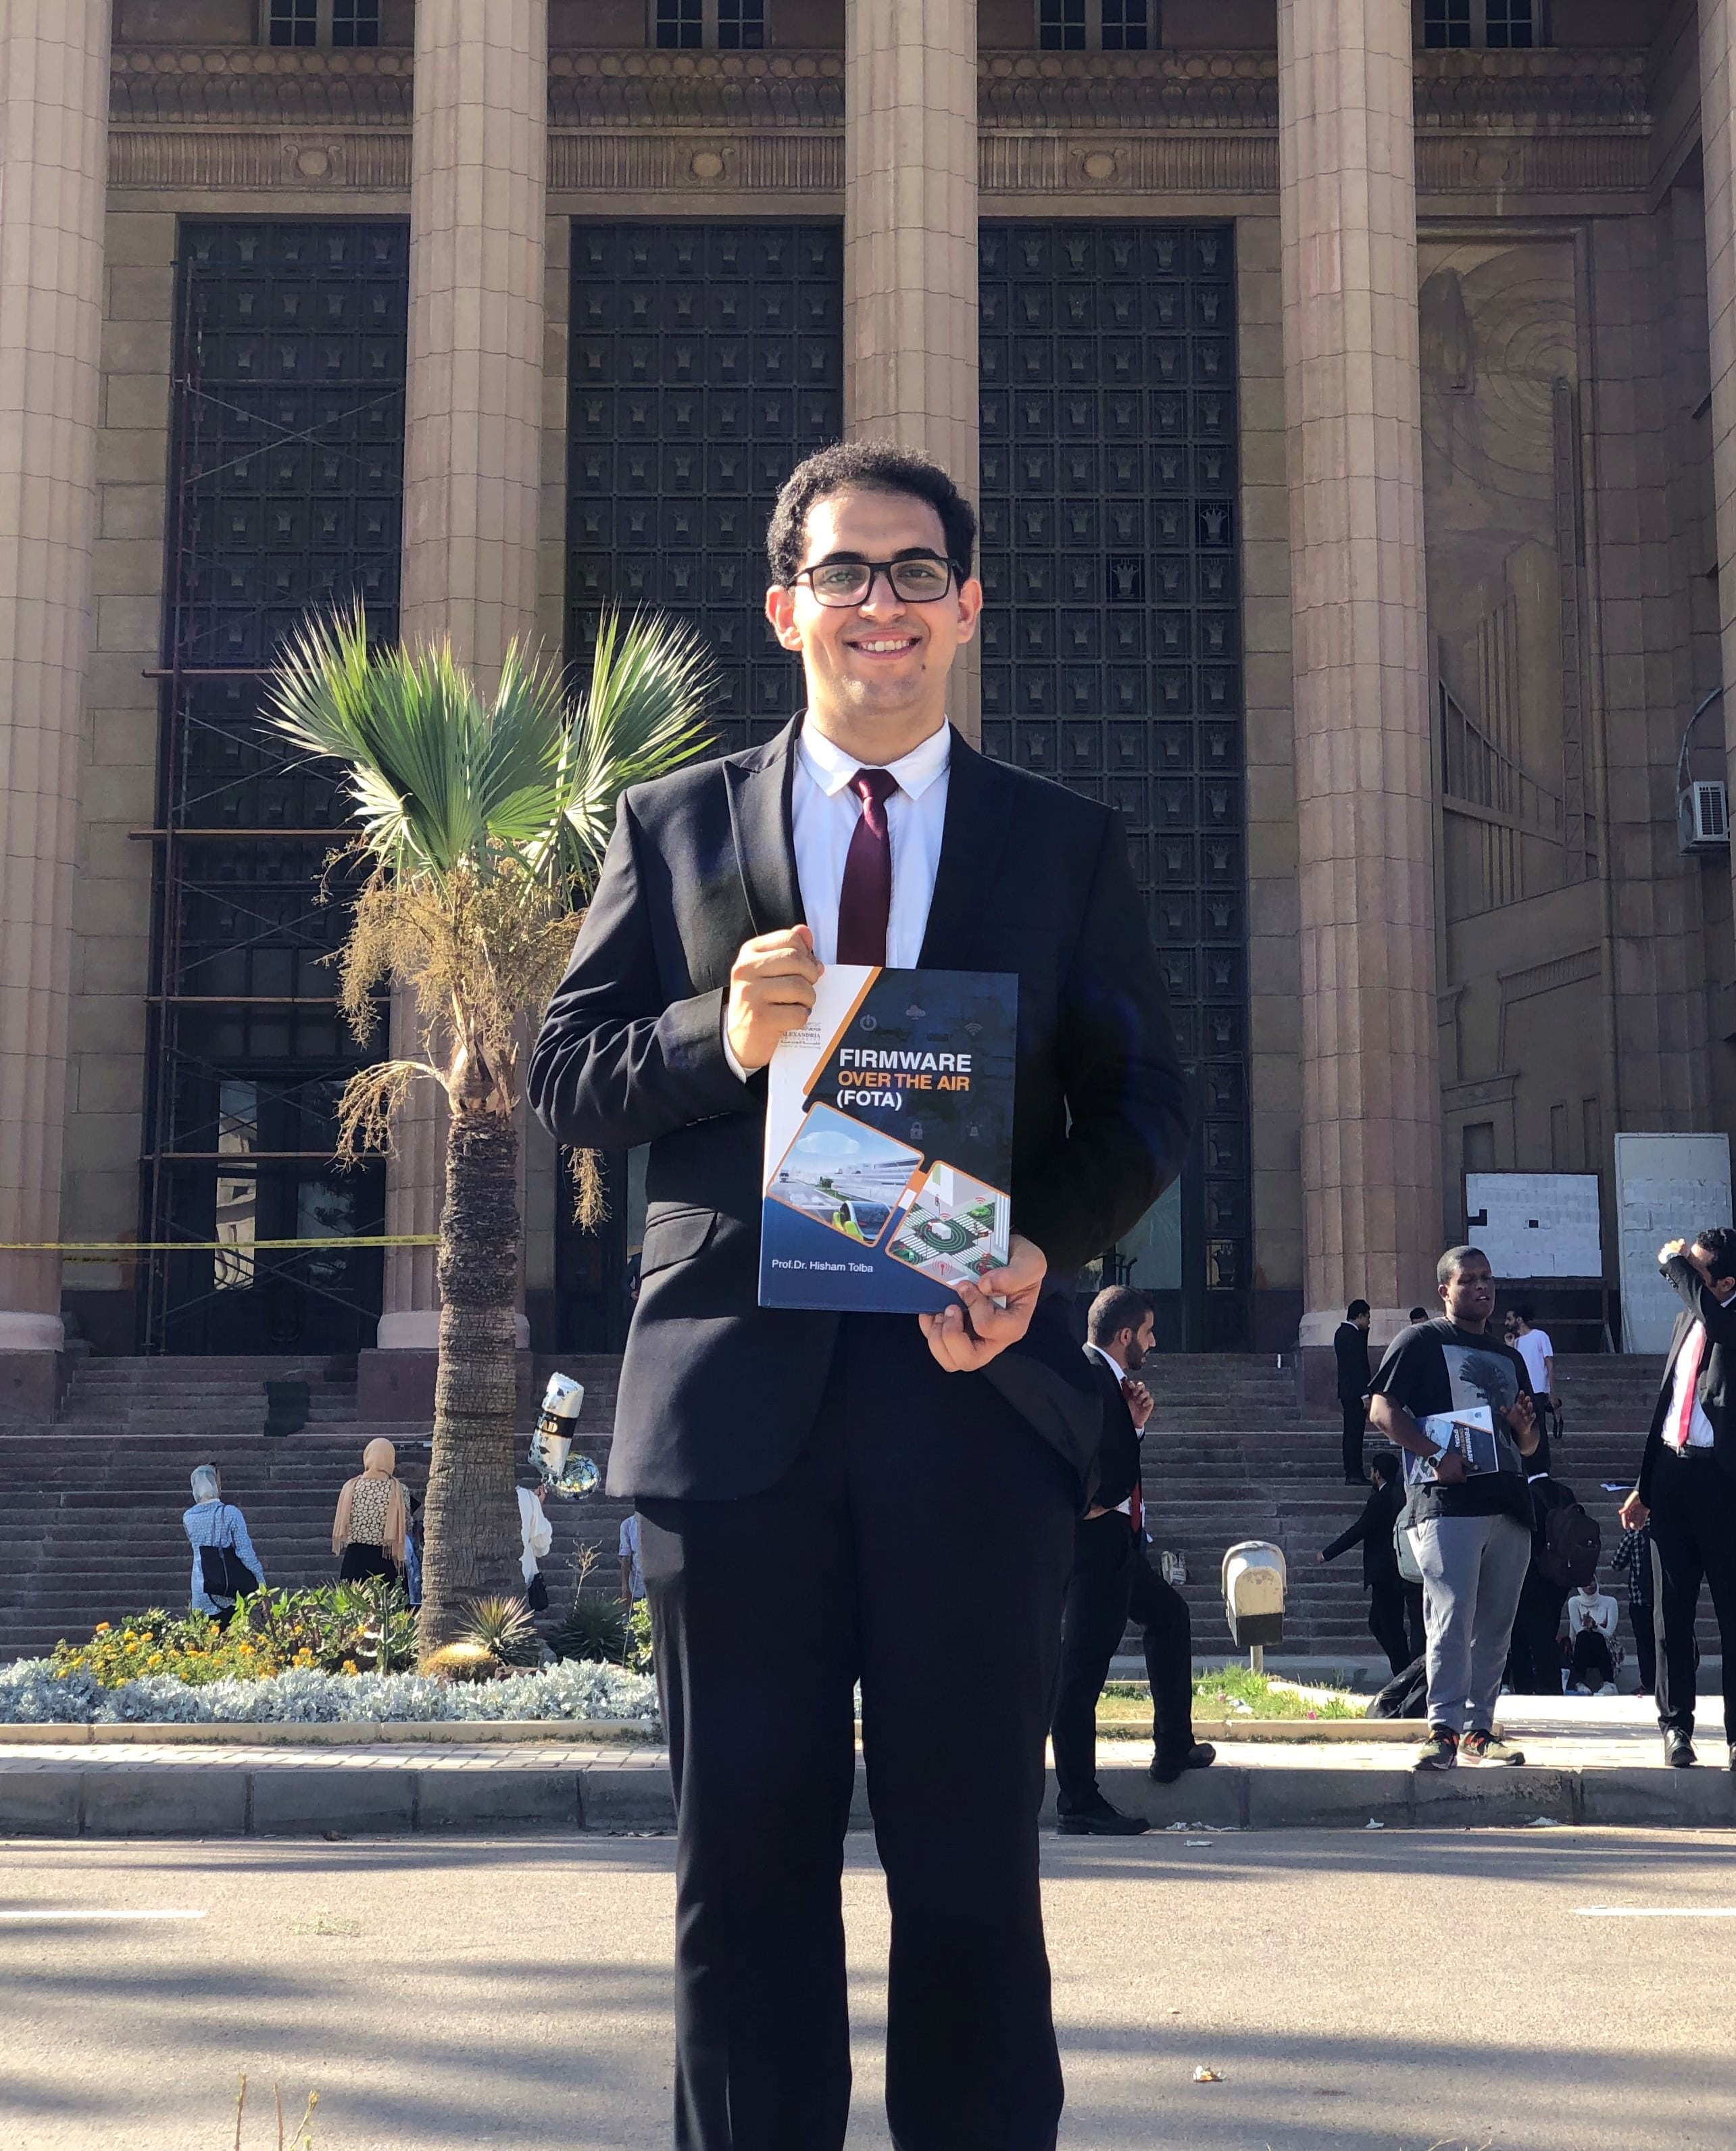
\includegraphics[width = .3\textwidth, height = .16\textheight]{Yehia Ehab}
\end{wrapfigure}
\textcolor{blue!40}{
\subsubsection{E- Reflections}}
“Torpedo team had a great impact on my life. This experience taught me a lot in my career. Also, it made me develop a winning mentality and changed my perspective on success. At Torpedo, we believe that our achievements come from the success of each member of our team”.  \\
-Yehia Ehab, Electrical Mentor. \\

\subsubsection{}
\begin{wrapfigure}{r}{.3\textwidth}
	\centering
	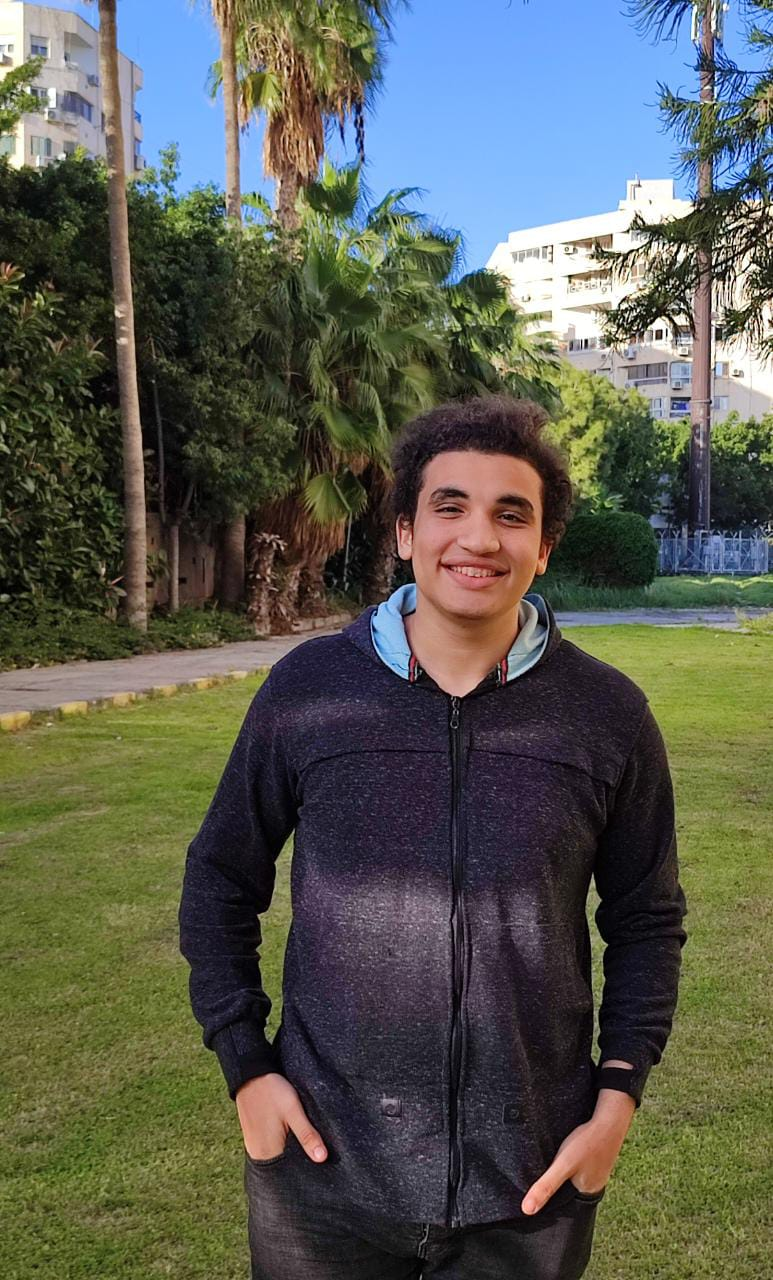
\includegraphics[width = .3\textwidth, height = .16\textheight]{Youssef Allam}
\end{wrapfigure}
“Knowledge is nothing without experience, and this is what I’ve been building since I joined the Torpedo team. The amazing people I met, the journey I went through, with its ups and downs, and the great things I learned, all of this is what makes joining Torpedo the best decision I have made this year, thanks to all the team”. \\
-Youssef Allam, Electrical Team member. \\
\subsubsection{}
\begin{wrapfigure}{r}{.3\textwidth}
	\centering
	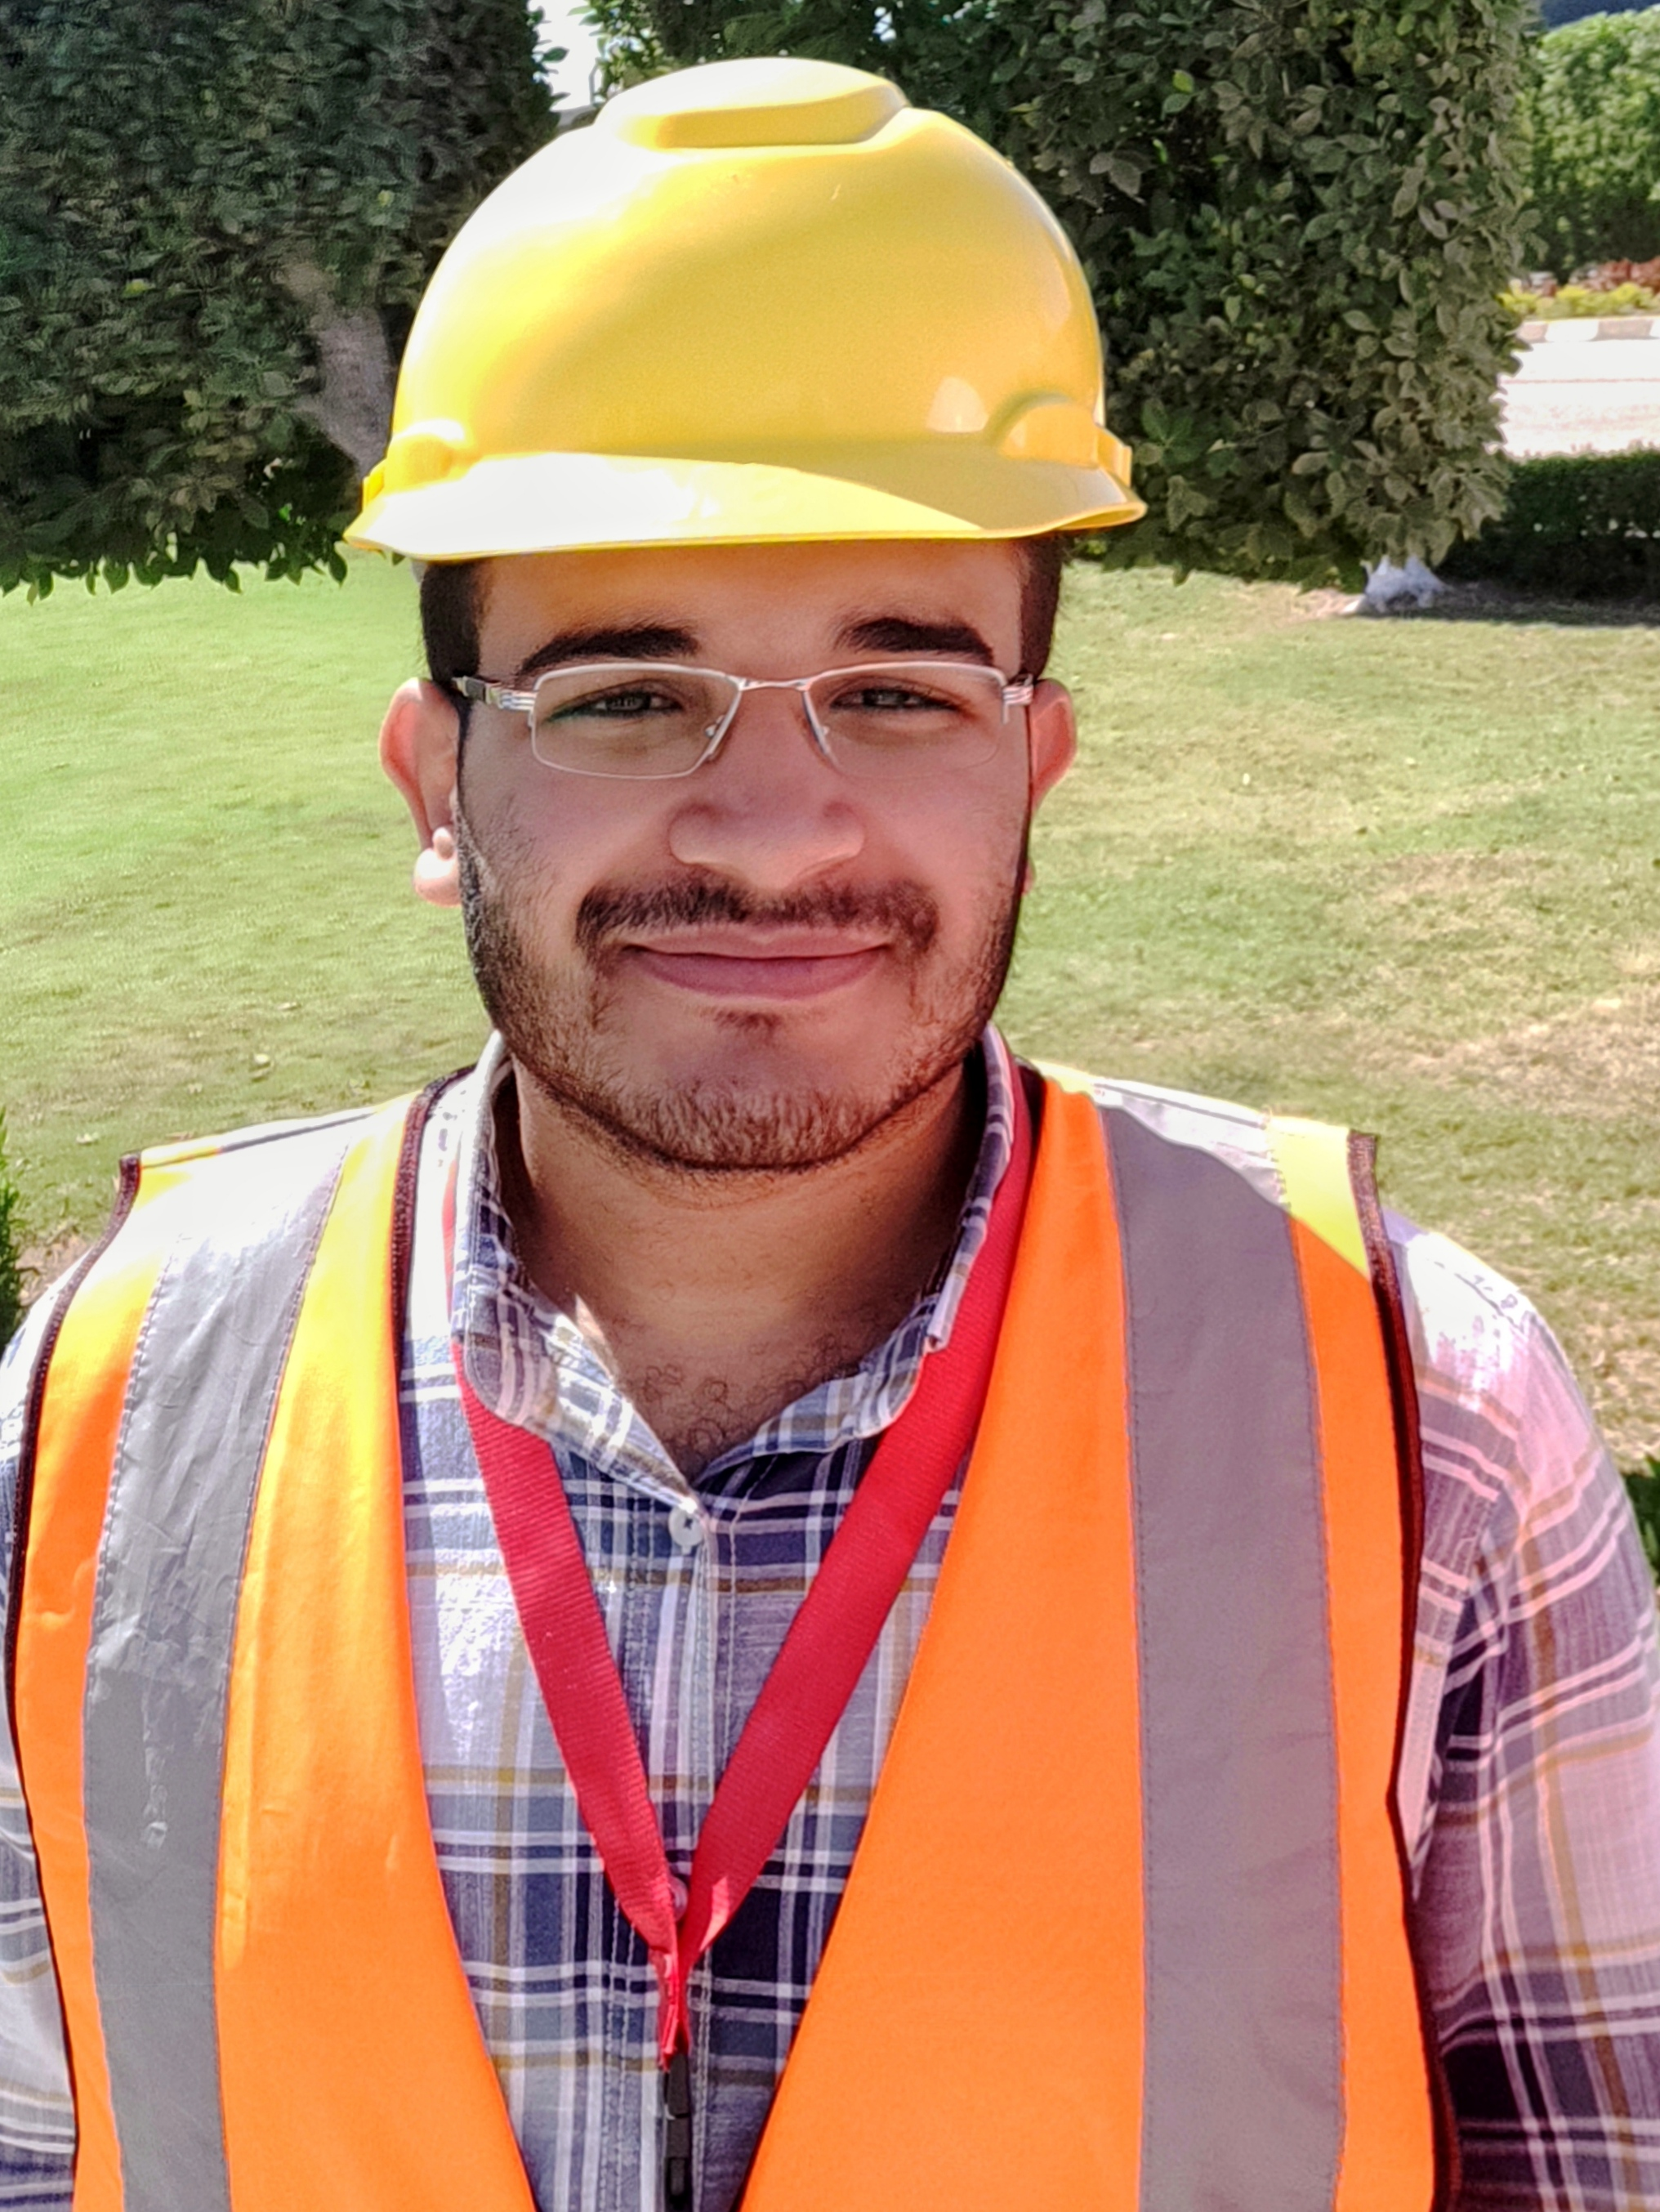
\includegraphics[width = .3\textwidth, height = .16\textheight]{Omar Al-lqany}
\end{wrapfigure}
The journey of being a mechanical member at Torpedo was like being in a family, and it helped me in so many ways, torpedo allowed me to try new ideas and to put my skills to the test, there was no fear of failing because we all knew that from failure comes success”. \\
-Omar Al-lqany, Mechanical Team Head.\\
 
\textcolor{blue!40}{
\subsubsection{F- Interpersonal Skills Gained}}
Our company relies on university students, throughout the journey of making Polaris they  learned how to manage their time between the college track and teamwork, due to the hardships  they encounter they managed to adapt to every possible situation and come out with the best  results of its which makes them push their potential beyond their limits since the company is  divided into two teams. They learned how to communicate with each other in an organized and  well-planned method to have the best outcome thus, the communication skills are Improved and  developed gradually. \\
\textcolor{blue!90}{
	\section{Appendices}}
\textcolor{blue!40}{
	\subsubsection{1- Cost Analysis }}
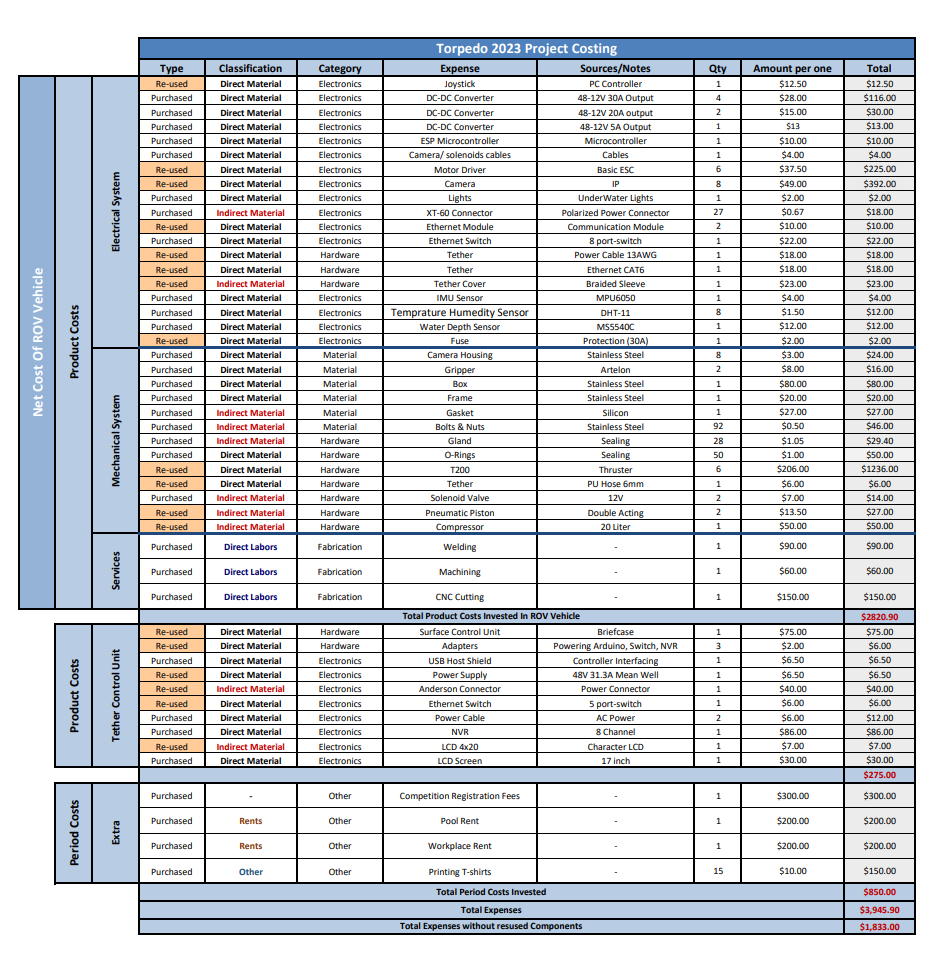
\includegraphics[width = \textwidth, height =.9\textheight]{Cost_analysis}

\end{document}